%Version 3.1 December 2024
% See section 11 of the User Manual for version history
%
%%%%%%%%%%%%%%%%%%%%%%%%%%%%%%%%%%%%%%%%%%%%%%%%%%%%%%%%%%%%%%%%%%%%%%
%%                                                                 %%
%% Please do not use \input{...} to include other tex files.       %%
%% Submit your LaTeX manuscript as one .tex document.              %%
%%                                                                 %%
%% All additional figures and files should be attached             %%
%% separately and not embedded in the \TeX\ document itself.       %%
%%                                                                 %%
%%%%%%%%%%%%%%%%%%%%%%%%%%%%%%%%%%%%%%%%%%%%%%%%%%%%%%%%%%%%%%%%%%%%%

%%\documentclass[referee,sn-basic]{sn-jnl}% referee option is meant for double line spacing

%%=======================================================%%
%% to print line numbers in the margin use lineno option %%
%%=======================================================%%

%%\documentclass[lineno,pdflatex,sn-basic]{sn-jnl}% Basic Springer Nature Reference Style/Chemistry Reference Style

%%=========================================================================================%%
%% the documentclass is set to pdflatex as default. You can delete it if not appropriate.  %%
%%=========================================================================================%%

%%\documentclass[sn-basic]{sn-jnl}% Basic Springer Nature Reference Style/Chemistry Reference Style

%%Note: the following reference styles support Namedate and Numbered referencing. By default the style follows the most common style. To switch between the options you can add or remove �Numbered� in the optional parenthesis. 
%%The option is available for: sn-basic.bst, sn-chicago.bst%  
 
%%\documentclass[pdflatex,sn-nature]{sn-jnl}% Style for submissions to Nature Portfolio journals
%%\documentclass[pdflatex,sn-basic]{sn-jnl}% Basic Springer Nature Reference Style/Chemistry Reference Style
\documentclass[pdflatex,sn-mathphys-num]{sn-jnl}% Math and Physical Sciences Numbered Reference Style
%%\documentclass[pdflatex,sn-mathphys-ay]{sn-jnl}% Math and Physical Sciences Author Year Reference Style
%%\documentclass[pdflatex,sn-aps]{sn-jnl}% American Physical Society (APS) Reference Style
%%\documentclass[pdflatex,sn-vancouver-num]{sn-jnl}% Vancouver Numbered Reference Style
%%\documentclass[pdflatex,sn-vancouver-ay]{sn-jnl}% Vancouver Author Year Reference Style
%%\documentclass[pdflatex,sn-apa]{sn-jnl}% APA Reference Style
%%\documentclass[pdflatex,sn-chicago]{sn-jnl}% Chicago-based Humanities Reference Style

%%%% Standard Packages
%%<additional latex packages if required can be included here>

\PassOptionsToPackage{table,xcdraw}{xcolor}
\usepackage{graphicx}%
\usepackage{multirow}%
\usepackage{amsmath,amssymb,amsfonts}%
\usepackage{amsthm}%
\usepackage{mathrsfs}%
\usepackage[title]{appendix}%
\usepackage{xcolor}%
\usepackage{textcomp}%
\usepackage{manyfoot}%
\usepackage{booktabs}%
\usepackage{algorithm}%
\usepackage{algorithmicx}%
\usepackage{algpseudocode}%
\usepackage{listings}%
\usepackage[most]{tcolorbox}
\usepackage{booktabs}
\usepackage{tabularx}
\usepackage{float}

\lstdefinelanguage{json}{
    basicstyle=\ttfamily\footnotesize,
    %%numbers=left,
    %%numberstyle=\tiny\color{gray},
    stepnumber=1,
    numbersep=5pt,
    showstringspaces=false,
    breaklines=true,
    frame=single,
    backgroundcolor=\color{gray!10},
    literate=
     *{0}{{{\color{blue}0}}}{1}
      {1}{{{\color{blue}1}}}{1}
      {2}{{{\color{blue}2}}}{1}
      {3}{{{\color{blue}3}}}{1}
      {4}{{{\color{blue}4}}}{1}
      {5}{{{\color{blue}5}}}{1}
      {6}{{{\color{blue}6}}}{1}
      {7}{{{\color{blue}7}}}{1}
      {8}{{{\color{blue}8}}}{1}
      {9}{{{\color{blue}9}}}{1}
}
\lstset{
  basicstyle=\ttfamily\footnotesize,
  breaklines=true,
%%  backgroundcolor=\color{blue!5}
  %%frame=single,
  numbers=none,
}
\tcbset{
    mypromptbox/.style={
        colback=blue!5,        % light blue background
        colframe=blue!80!black, % blue border
        boxrule=0.5pt,         % border thickness
        arc=4pt,               % rounded corners
        outer arc=4pt,
        boxsep=5pt,            % padding inside box
        left=5pt,
        right=5pt,
        top=5pt,
        bottom=5pt,
        breakable              % allow page breaks inside box
    }
}

%%%%

%%%%%=============================================================================%%%%
%%%%  Remarks: This template is provided to aid authors with the preparation
%%%%  of original research articles intended for submission to journals published 
%%%%  by Springer Nature. The guidance has been prepared in partnership with 
%%%%  production teams to conform to Springer Nature technical requirements. 
%%%%  Editorial and presentation requirements differ among journal portfolios and 
%%%%  research disciplines. You may find sections in this template are irrelevant 
%%%%  to your work and are empowered to omit any such section if allowed by the 
%%%%  journal you intend to submit to. The submission guidelines and policies 
%%%%  of the journal take precedence. A detailed User Manual is available in the 
%%%%  template package for technical guidance.
%%%%%=============================================================================%%%%

%% as per the requirement new theorem styles can be included as shown below
\theoremstyle{thmstyleone}%
\newtheorem{theorem}{Theorem}%  meant for continuous numbers
%%\newtheorem{theorem}{Theorem}[section]% meant for sectionwise numbers
%% optional argument [theorem] produces theorem numbering sequence instead of independent numbers for Proposition
\newtheorem{proposition}[theorem]{Proposition}% 
%%\newtheorem{proposition}{Proposition}% to get separate numbers for theorem and proposition etc.

\theoremstyle{thmstyletwo}%
\newtheorem{example}{Example}%
\newtheorem{remark}{Remark}%

\theoremstyle{thmstylethree}%
\newtheorem{definition}{Definition}%

\raggedbottom
%%\unnumbered% uncomment this for unnumbered level heads

\begin{document}

\title[Article Title]{MediSyn: A Synergistic multi-agent AI system for IPE in medical domain}

%%=============================================================%%
%% GivenName	-> \fnm{Joergen W.}
%% Particle	-> \spfx{van der} -> surname prefix
%% FamilyName	-> \sur{Ploeg}
%% Suffix	-> \sfx{IV}
%% \author*[1,2]{\fnm{Joergen W.} \spfx{van der} \sur{Ploeg} 
%%  \sfx{IV}}\email{iauthor@gmail.com}
%%=============================================================%%

\author*[1]{\fnm{Sajan K.} \sur{Kar}}\email{sajan.kar@gwu.edu}
\equalcont{These authors contributed equally to this work.}

\author*[2]{\fnm{Parv} \sur{Bhargava}}\email{parv.bhargava@gwu.edu}
\equalcont{These authors contributed equally to this work.}

\author[3]{\fnm{Amir} \sur{Jafari}}\email{ajafari@gwu.edu}


\affil*[1]{\orgdiv{Data Science Program}, \orgname{George Washington University}, \orgaddress{\street{2121 I St NW}, \city{Washington D.C.}, \postcode{20052}, \state{DC}, \country{USA}}}

\affil*[2]{\orgdiv{Data Science Program}, \orgname{George Washington University}, \orgaddress{\street{2121 I St NW}, \city{Washington D.C.}, \postcode{20052}, \state{DC}, \country{USA}}}

\affil[3]{\orgdiv{Data Science Program}, \orgname{George Washington University}, \orgaddress{\street{2121 I St NW}, \city{Washington D.C.}, \postcode{20052}, \state{DC}, \country{USA}}}

%%==================================%%
%% Sample for unstructured abstract %%
%%==================================%%

\abstract{The increasing complexity of modern healthcare necessitates collaborative, inter-professional approaches to ensure comprehensive patient care. While general-purpose large language models (LLMs) offer promising capabilities, they often lack the profession-specific reasoning needed for clinically grounded treatment planning. In this work, we explore the integration of Inter-Professional Education/Practice (IPE/IPP) principles into an AI-driven framework by developing MediSyn—a multi-agent system that dynamically creates role-specific agents based on real-world case studies. We compare this approach against baseline methods including single LLM and prompt-tuned LLM pipelines, each tasked with generating treatment plans from structured case data. Rather than asserting a singular best-performing solution, our aim is to evaluate how a specialized multi-agent design stacks up against more general-purpose strategies. The findings offer valuable insights into the trade-offs between domain-informed agent collaboration and general LLM-based approaches in medical AI applications.}

%%================================%%
%% Sample for structured abstract %%
%%================================%%

% \abstract{\textbf{Purpose:} The abstract serves both as a general introduction to the topic and as a brief, non-technical summary of the main results and their implications. The abstract must not include subheadings (unless expressly permitted in the journal's Instructions to Authors), equations or citations. As a guide the abstract should not exceed 200 words. Most journals do not set a hard limit however authors are advised to check the author instructions for the journal they are submitting to.
% 
% \textbf{Methods:} The abstract serves both as a general introduction to the topic and as a brief, non-technical summary of the main results and their implications. The abstract must not include subheadings (unless expressly permitted in the journal's Instructions to Authors), equations or citations. As a guide the abstract should not exceed 200 words. Most journals do not set a hard limit however authors are advised to check the author instructions for the journal they are submitting to.
% 
% \textbf{Results:} The abstract serves both as a general introduction to the topic and as a brief, non-technical summary of the main results and their implications. The abstract must not include subheadings (unless expressly permitted in the journal's Instructions to Authors), equations or citations. As a guide the abstract should not exceed 200 words. Most journals do not set a hard limit however authors are advised to check the author instructions for the journal they are submitting to.
% 
% \textbf{Conclusion:} The abstract serves both as a general introduction to the topic and as a brief, non-technical summary of the main results and their implications. The abstract must not include subheadings (unless expressly permitted in the journal's Instructions to Authors), equations or citations. As a guide the abstract should not exceed 200 words. Most journals do not set a hard limit however authors are advised to check the author instructions for the journal they are submitting to.}

\keywords{Multi-agent system, LLM, Inter-professional, Collaborative, IPE, IPP, Healthcare, AI}

%%\pacs[JEL Classification]{D8, H51}

%%\pacs[MSC Classification]{35A01, 65L10, 65L12, 65L20, 65L70}

\maketitle

\section{Introduction}\label{sec1}

In modern healthcare, the complexity of patient needs necessitates collaborative approaches among diverse healthcare professionals. Interprofessional Education (IPE), as defined by the World Health Organization (WHO), occurs when ``students from two or more professions learn about, from and with each other to enable effective collaboration and improve health outcomes''~\cite{WHO2010}. Building upon this educational foundation, Interprofessional Practice (IPP) involves ``multiple health workers from different professional backgrounds working together with patients, families, carers, and communities to deliver the highest quality of care''~\cite{WHO2010}. These practices have been shown to enhance communication, reduce medical errors, and improve clinical effectiveness by aligning profession-specific expertise toward common goals.


With the emergence of large language models (LLMs) in medical AI applications, there is growing interest in leveraging their capabilities to support or simulate such interprofessional reasoning. However, general-purpose LLMs often lack the role awareness and domain-specific context needed to replicate nuanced clinical decision-making, especially in multi-role environments. These models typically produce generic treatment plans that may overlook profession-specific insights critical to comprehensive patient care.

In this work, we investigate how different LLM-based approaches perform in generating treatment plans for real-world IPE case studies. Specifically, we compare three paradigms: (1) a single general-purpose LLM, (2) a prompt-tuned LLM, and (3) \textit{MediSyn} — a novel AI-driven multi-agent system that simulates an interprofessional care team by dynamically instantiating specialized agents for each role mentioned in a case. Rather than hardcoding professions, MediSyn parses the team members from the input and assigns each agent domain-specific responsibilities. For example, a nurse agent is fine-tuned to provide insights into patient care, while an oncologist agent delivers targeted cancer treatment recommendations.

Importantly, our goal is not to position MediSyn as a universally superior alternative, but rather to explore how such a system compares to more general-purpose LLM pipelines. We ask: \textit{Can simulating interprofessional dynamics through a role-specialized multi-agent framework provide advantages — or trade-offs — relative to current monolithic approaches?}

Moreover, our extensive review of the current literature and AI applications in healthcare indicates that, although there are various multi-agent systems addressing tasks such as emergency response~\cite{han2024development}, interdisciplinary decision support~\cite{wilk2016semantic}, and cancer care information management~\cite{mohammadzadeh2013multi}, no existing system to our knowledge has been designed to tackle real IPE case studies using generative AI.

Through this work, we aim to provide empirical insights into the capabilities and limitations of these AI paradigms in replicating interprofessional treatment planning, and inform the design of future AI systems for interprofessional healthcare collaboration.

The remainder of this paper is organized as follows: Section~\ref{sec2} reviews related work on AI-driven medical systems, multi-agent approaches, and LLMs in healthcare. Section~\ref{sec3} describes our methodology, including the dataset, preprocessing strategies, baseline generation pipelines, and the design of the MediSyn framework. Section~\ref{sec4} presents our experimental results comparing single LLM, prompt-tuned LLM, and multi-agent outputs across multiple evaluation metrics. Section~\ref{sec5} discusses key insights, limitations, and open challenges. Finally, Section~\ref{sec6} concludes the paper and suggests directions for future work.


\section{Related Work}\label{sec2}

The integration of large language models (LLMs) in healthcare has spurred growing interest in their use for tasks such as clinical decision support, treatment recommendation, and patient education~\cite{singhal2023gpt4med, biswas2023role, patel2023chatgpt, nori2023capabilities}. While models like GPT-3 and GPT-4 have demonstrated impressive capabilities in understanding and generating medical language~\cite{lee2023benefits, li2023can}, they often lack the role-specific contextual awareness necessary for profession-targeted treatment planning~\cite{valmeek2023prompt}. Their responses may be overly generic, missing the nuanced reasoning that emerges from collaborative healthcare practice involving diverse specialties.

To better address distributed reasoning, multi-agent systems (MAS) have been explored extensively in healthcare.MAS architectures simulate collaboration by assigning responsibilities to individual agents representing different medical roles~\cite{ghazal2014multiagent, lemke2011agent, abidi2017ontology}.. Applications include chronic disease management, prehospital triage, cancer care coordination, and emergency response systems. These systems enable real-time communication, adaptive decision-making, and decentralized control — making them well-suited for modeling complex healthcare processes~\cite{lemke2011agent, abidi2017ontology}.

The emergence of LLM-powered MAS frameworks bridges the gap between generative text reasoning and collaborative simulation. For instance, ClinicalAgent~\cite{wang2024clinicalagent} demonstrates the use of GPT-4-based agents for simulating clinical trial coordination, where each agent is assigned a domain-specific function, such as patient recruitment or outcome analysis. Similarly, Han and Choi~\cite{han2024development} developed an LLM-based multi-agent system for emergency triage using the Korean Triage and Acuity Scale (KTAS), dynamically orchestrating agents like triage nurse, physician, and coordinator for treatment planning. These systems highlight the growing feasibility of combining natural language understanding with agent-based role simulation in medicine.

Recent advancements have introduced sophisticated LLM-based multi-agent frameworks tailored for complex medical tasks. For instance, the KG4Diagnosis system integrates hierarchical agents with knowledge graphs to enhance diagnostic reasoning across various medical specialties.~\cite{kg4diagnosis2024} Similarly, the MedAide framework employs specialized agents collaborating through retrieval-augmented generation to provide personalized healthcare services.~\cite{medaide2024} The MDAgents platform emphasizes adaptive collaboration among expert LLMs to tackle intricate medical decision-making processes.~\cite{mdagents2024} Furthermore, the Multi-Agent Conversation (MAC) framework has demonstrated significant improvements in diagnostic accuracy by simulating collaborative discussions among agents.~\cite{macframework2025} These innovations underscore the potential of multi-agent LLM systems to replicate the collaborative dynamics of healthcare professionals, offering promising avenues for enhancing clinical decision support.

However, existing work has not yet addressed interprofessional education (IPE) or interprofessional practice (IPP) case studies using generative AI in a fully dynamic, role-adaptive way. Most prior systems rely on static agent configurations, do not reflect the diversity of real-world care teams, or are not designed for educational or collaborative training contexts~\cite{wilk2016semantic, valmeek2023prompt}. Our work builds upon these foundations by introducing MediSyn, an LLM-powered multi-agent system that dynamically extracts team roles from real IPE case studies and assigns them to profession-specialized agents. Rather than aiming to outperform prior methods, we explore how this novel architecture compares to single-LLM and prompt-tuned LLM baselines in generating treatment plans, particularly in scenarios requiring collaborative, role-sensitive reasoning.


\section{Methodology}\label{sec3}

This section provides an overview of the methodology adopted in this work. Our approach is designed to evaluate the performance of a novel multi-agent AI system, \textit{MediSyn}, for generating treatment plans in Interprofessional Education (IPE) healthcare scenarios. The methodology involves a structured pipeline, progressing from data extraction and preprocessing to various LLM-based generation approaches, culminating in the design and evaluation of the proposed multi-agent framework.

At a high level, our methodology can be divided into the following major components:

\begin{itemize} \item \textbf{Data Collection:} We source our data from 18 publicly available healthcare case studies provided by the American Speech-Language-Hearing Association (ASHA). These case studies serve as authentic real-world examples of interprofessional collaboration in healthcare settings.
\item \textbf{Data Preprocessing:} The unstructured case study narratives are processed into a structured JSON format suitable for LLM input. This involves both manual extraction and automated extraction using LLMs, allowing us to compare the effectiveness of both approaches.

\item \textbf{Baseline Approaches:} We establish two baseline methods for treatment plan generation:
\begin{enumerate}
    \item A \textit{Single LLM} pipeline where the entire case study is passed to a general-purpose LLM (like GPT-4 or Claude) to generate a treatment plan.
    \item A \textit{Prompt-Tuned LLM} pipeline where the prompt is carefully crafted to simulate specific roles or expectations from the model.
\end{enumerate}

\item \textbf{MediSyn: Proposed Multi-Agent System:} Moving beyond single LLM baselines, we introduce MediSyn, a novel synergistic multi-agent architecture. For each case study, MediSyn dynamically identifies the healthcare team members mentioned and creates specialized agents — each representing a profession involved in the case. These agents are constrained to their domain knowledge and collaborate sequentially to generate the final treatment plan, thereby closely simulating real-world interprofessional collaboration.

\item \textbf{Evaluation Metrics:} To rigorously evaluate and compare the outputs of the Single LLM, Prompt-Tuned LLM, and MediSyn systems, we employ both automated and human-centric evaluation methods:
\begin{itemize}
    \item BLEU Score
    \item ROUGE Score
    \item LLM-as-a-Judge evaluations (for qualitative and contextual judgment)
\end{itemize}
\end{itemize}

\subsection{Data Description}\label{subsec3.1}

The dataset used in this study consists of a curated collection of real-world healthcare case studies sourced from the American Speech-Language-Hearing Association (ASHA) \cite{asha}. These case studies are publicly available on the ASHA IPE/IPP portal and are specifically designed to highlight examples of interprofessional collaboration across diverse healthcare scenarios. 

Each case study presents a unique clinical situation involving patients from varying demographics and medical backgrounds, including conditions such as cleft palate, traumatic brain injury, autism spectrum disorder, NICU interventions, and rehabilitation settings. Importantly, each case involves a multidisciplinary team working together to provide holistic patient care. Every case study in this dataset typically contains:
\begin{itemize}
    \item A clinical background of the patient
    \item A list of healthcare team members involved (e.g., Nurse, Physician, Speech-Language Pathologist, Audiologist, Occupational Therapist)
    \item The collaborative assessment process and challenges faced
    \item The treatment plan co-developed by the team
    \item Patient outcomes and post-intervention progress
\end{itemize} 
\begin{figure}[h]
    \centering
    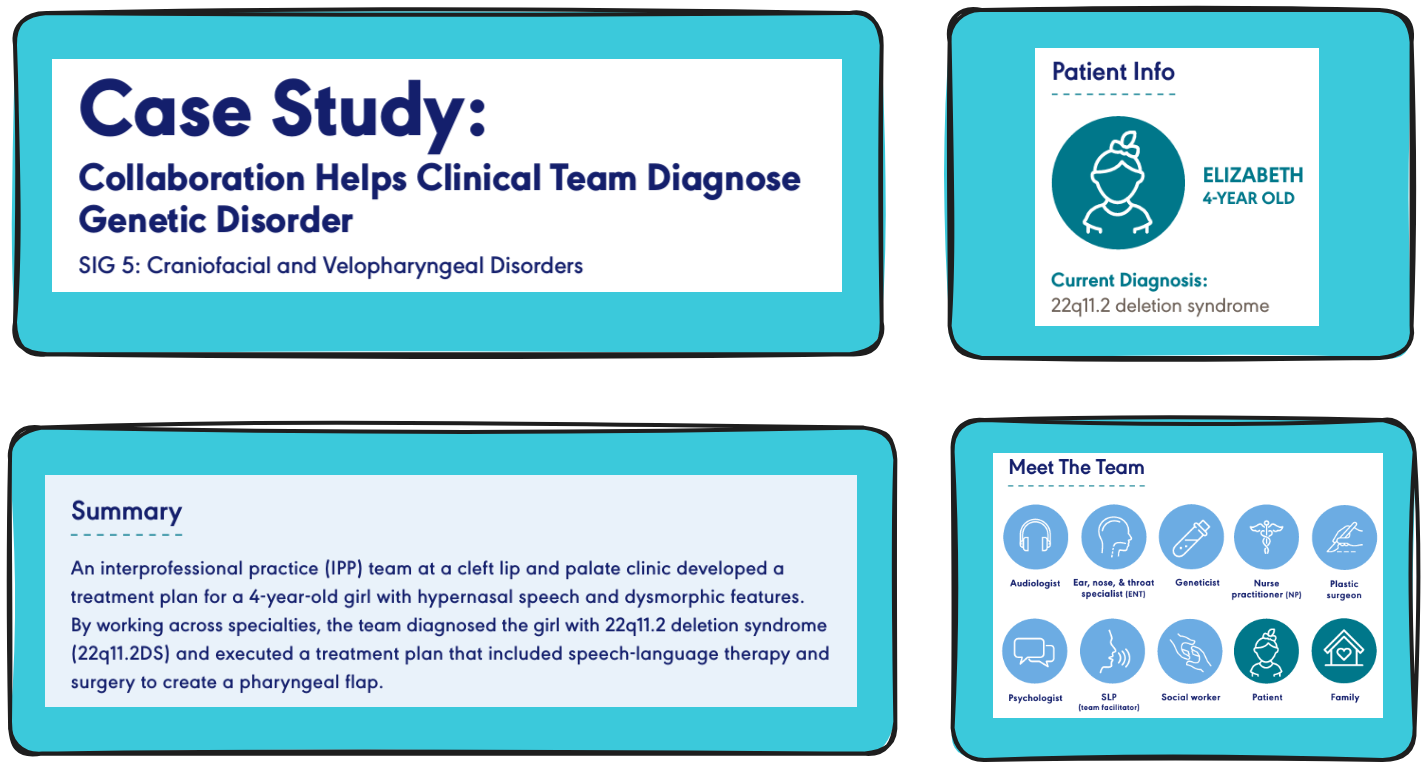
\includegraphics[width=0.85\textwidth]{Fig/data1.png}
    \caption{\centering 1st page of the case study with Patient Info, summary, and the team members}
    \label{fig:Case study (1st page)}
\end{figure}

The above diagram is a view of some of the elements in one particular case study. Each ASHA case study follows a more-or-less consistent structure comprising several distinct sections or headers, namely: \begin{itemize} \item \textbf{Summary:} A brief narrative of the case and its significance. \item \textbf{Patient Info:} Demographic and clinical details about the patient. \item \textbf{Meet The Team:} List of interprofessional healthcare team members involved. \item \textbf{Background:} Detailed description of the patient's history, presenting problems, and symptoms. \item \textbf{How They Collaborated:} A narrative explanation of the collaborative process among team members. \item \textbf{Outcome:} The outcome of the case. \item \textbf{Ongoing collaboration:} Whether the team is still involved in the process of treatment or in the patient's care. \item \textbf{History and Concerns:} Essentially a copy of the background section. \item \textbf{Assessment Plan:} The roles and responsibilities of each professional in evaluating the patient. \item \textbf{Assessment Results:} Key diagnostic findings from each professional’s evaluation. \item \textbf{IPP Treatment Plan:} The final collaboratively agreed treatment plan. \item \textbf{Treatment Outcomes:} Follow-up details on patient progress. \item \textbf{Team Follow-Up:} Plan for continued interprofessional communication and monitoring. \end{itemize}
To understand the features better, here's a snapshot of the raw data:
\begin{figure}[h]
    \centering
    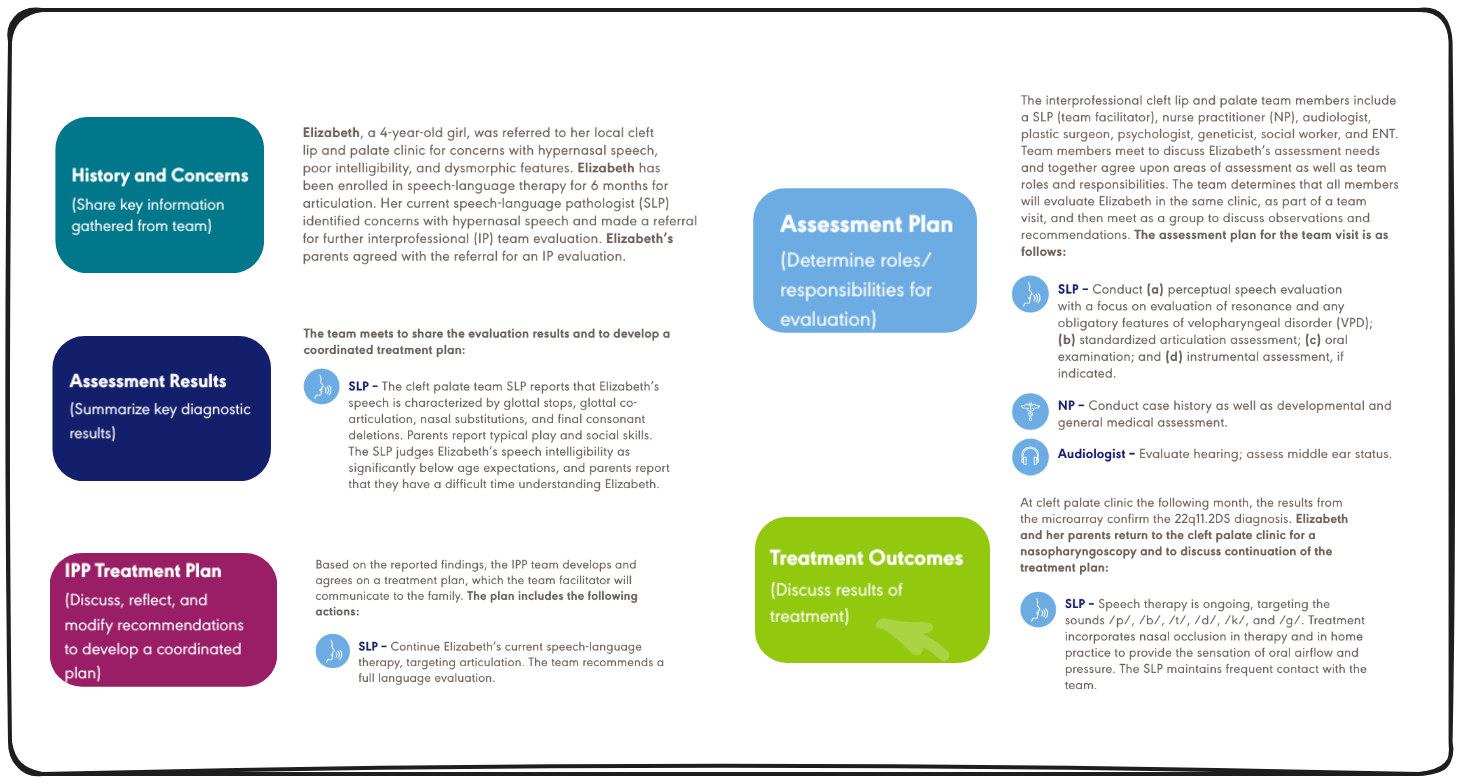
\includegraphics[width=0.8\textwidth]{Fig/data3.png}
    \caption{\centering Data Features}
    \label{fig:Case study (Features)}
\end{figure}

In total, the dataset contains 18 such case studies. These cases serve two main purposes in our research:
\begin{enumerate}
    \item As input data for generating treatment plans using baseline single LLM approaches.
    \item As structured case scenarios for instantiating profession-specific agents within the MediSyn multi-agent framework.
\end{enumerate}

Out of the 18 case studies available at the time of our work, we utilized 15 case studies for our experiments. The remaining 3 case studies were excluded from our analysis due to the absence of a documented Interprofessional Practice (IPP) treatment plan and a few other parts, which are critical components for our evaluation and generation pipeline.
This dataset is highly suitable for simulating IPE scenarios as it authentically captures real-world interprofessional teamwork, role-specific responsibilities, and collaborative decision-making processes — all of which are essential for modeling and evaluating agentic behavior in our proposed system.


\subsection{Data Preprocessing}\label{subsec3.2}

Now that we have talked about the various features that a case study has. For the purpose of our work, we identified and extracted the follwing essential features from each case study, which directly support the downstream treatment plan generation and multi-agent modeling tasks:

\begin{table}[h]
\centering
\caption{Extracted Fields}
\renewcommand{\arraystretch}{1.3} % row height
\rowcolors{2}{blue!5}{white}     % alternate row colors
\begin{tabularx}{\textwidth}{|l|X|}
\toprule
\rowcolor{blue!15}
\texttt{Field} & \textbf{Description} \\
\midrule
\texttt{patient\_info}       & Includes patient's name, age, and diagnosis. \\
\texttt{summary}             & Summary of the case. \\
\texttt{team\_members}       & List of involved professionals (Meet the Team section). \\
\texttt{background}          & Patient's background. \\
\texttt{assessment\_plan}    & Evaluation responsibilities assigned to each professional (Assessment Plan section). \\
\texttt{assessment\_results} & Results of diagnostic evaluations (Assessment Results section). \\
\texttt{treatment\_plan}     & The final Interprofessional Practice (IPP) treatment plan co-developed by the team (IPP Treatment Plan section). \\
\bottomrule
\end{tabularx}
\label{tab:extracted_fields}
\end{table}


The extracted information was organized into a clean JSON structure as shown below:
\begin{lstlisting}[language=json, caption={Structure of extracted JSON from case study}, linewidth=\textwidth]
{
  "patient_info": {
    ...
  },
  "summary": "...",
  "team_members": [
    ...
  ],
  "background": "...",
  "assessment_plan": "...",
  "assessment_results": "...",
  "treatment_plan": "..."
}
\end{lstlisting}

This structured representation enables a standardized and consistent input format for all subsequent methods — including baseline LLM approaches and our proposed MediSyn multi-agent system. Thing to note is the treatment plan is our target feature.

To transform the ASHA case studies into a structured format suitable for downstream LLM processing and multi-agent generation, we employed two complementary data preprocessing strategies: (1) manual extraction, and (2) automated extraction using LLMs. These pipelines enabled consistent representation of each case study while also facilitating a comparison between human- and machine-curated inputs.

\subsubsection{Manual}\label{subsec3.2.1}

In the manual preprocessing approach, the data from each ASHA case study was directly extracted from the raw PDF files without any alterations or modifications. Specifically, the relevant sections corresponding to the identified features were carefully copy-pasted from the case studies and structured into JSON format as described earlier.

This method ensures that the extracted data maintains maximum fidelity to the original case study content, preserving the exact phrasing, structure, and information as presented in the source. The manually curated JSON files therefore serve as the most authentic representation of the data and act as the ground truth for comparison against automated methods.

This approach, while labor-intensive, was crucial in providing clean, reliable data for evaluating the performance of LLM-based extraction methods and the subsequent treatment plan generation.

\subsubsection{LLM}\label{subsec3.2.2}

In contrast to the manual extraction approach, we also explored an automated extraction pipeline using state-of-the-art Large Language Models (LLMs) to convert the ASHA case studies from raw PDFs into structured JSON format.

We utilized three different LLMs to perform this task: \begin{itemize} \item LLaMA 3.2 70B Instruct model (accessed via AWS Bedrock) \item Claude 3.5 Sonnet (accessed via AWS Bedrock) \item GPT-4o (accessed via OpenAI API) \end{itemize}

Each of these models was provided with the raw text extracted from the PDF files using unstructured library, along with a carefully crafted prompt instructing the model to extract all relevant information and output it in the exact JSON format described earlier. The prompt structure remained largely consistent across models, with minor adjustments specific to the respective LLM formatting requirements. The detailed design and content of the prompt used for this extraction process is discussed in Section~\ref{subsec4.1}.

\begin{figure}[H]
    \centering
    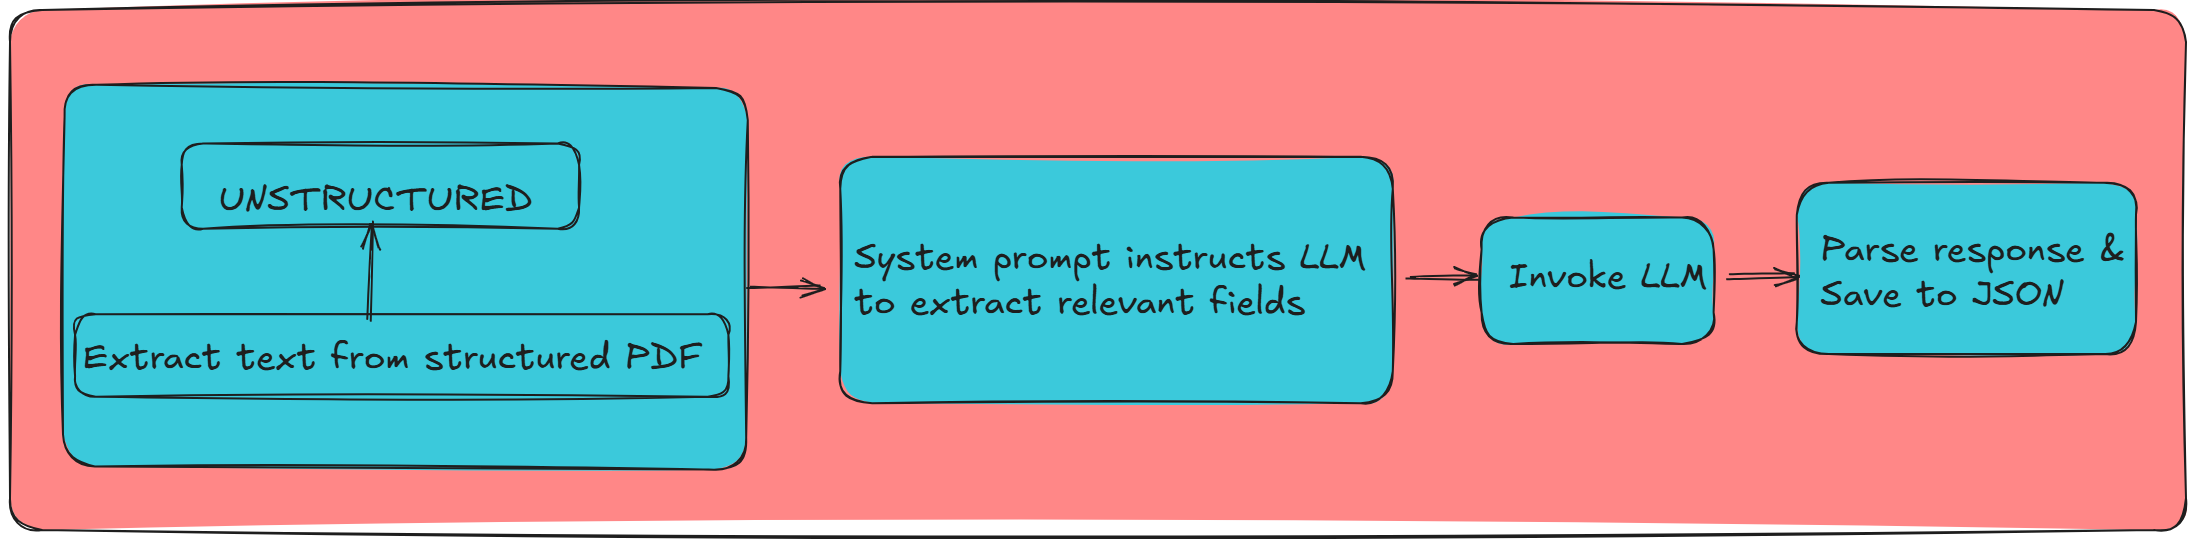
\includegraphics[width=1.0\textwidth]{Fig/data_extraction_process.png}
    \caption{\centering Data Extraction Process}
    \label{fig:data_ext}
\end{figure}
We leveraged a dedicated Python pipeline that involved extracting structured text from PDFs using the Unstructured library. A specialized system prompt was then created to instruct the model to extract specific fields, including patient info, summary, team members, background, assessment plan, assessment results, and treatment plan. This prompt was passed to the LLaMA 3.2 model deployed on AWS Bedrock via the Bedrock Runtime client. The generated response was parsed to extract valid JSON content, which was subsequently saved into a structured JSON file.

We repeated the same extraction process individually for all three models, thereby generating three separate sets of JSON files — one from each LLM.

Going forward, these generated datasets were exclusively used with their respective models for downstream treatment plan generation tasks. Specifically: \begin{itemize} \item LLaMA-generated JSONs were used as input when evaluating LLaMA's performance for treatment plan generation. \item Claude-generated JSONs were used with Claude for treatment generation. \item GPT-generated JSONs were used with GPT for treatment generation. \end{itemize}
The details are furthur explained in Sections~\ref{subsec4.2},~\ref{subsec4.3.2} and ~\ref{subsec4.4.2}

This design choice allowed us to maintain consistency in the data-model pairing while simultaneously evaluating the extraction and generation capabilities of each LLM independently.

\subsection{Single LLM}\label{subsec3.3}

As a foundational baseline, we first explored a straightforward single-LLM approach for treatment plan generation. In this method, a general-purpose large language model (LLM) is prompted with the structured case study data — in JSON format — and tasked with generating a comprehensive treatment plan for the patient described.

This approach serves two primary purposes:
(1) It establishes a baseline performance level for evaluating how well a single, monolithic LLM can handle interprofessional medical reasoning, and
(2) It allows us to contrast the effectiveness of centralized, undifferentiated AI decision-making with our proposed multi-agent collaborative system, MediSyn.

In the single-LLM setup, we use three different models for comparative analysis: \begin{itemize} \item GPT-4o (OpenAI) \item Claude 3.5 Sonnet (Anthropic via AWS Bedrock) \item LLaMA 3.2 70B Instruct (Meta via AWS Bedrock) \end{itemize}

Each model is provided the same structured input (case study JSON), which includes key components such as patient information, background, team members, assessment plan, and diagnostic results. The final field, the treatment plan, is left blank and is expected to be generated by the LLM itself based on the context provided in the other fields.

The system prompt instructs the model to act as a virtual care team, combining the insights of all team members to propose a unified treatment plan. The prompt also emphasizes clinical accuracy, role-sensitive insights, and realistic medical interventions. The specific prompts used for each LLM are documented in Section~\ref{subsec4.1}.

This single-model approach provides a valuable reference point for evaluating how general-purpose LLMs perform in the context of interprofessional treatment planning in healthcare decision-making, particularly when tasked with replicating the depth and nuance of interprofessional collaboration. As we demonstrate in our experimental results, while these models are capable of generating plausible treatment plans,they may lack the role-specific depth and collaborative dynamics found in interprofessional teams — which our multi-agent system is designed to simulate and explore.

\subsection{Prompt Tuned LLM}\label{subsec3.4}

To improve the performance of general-purpose large language models (LLMs) without altering their architecture, we explored a prompt-tuning strategy. In this approach, we continued using the same structured case study JSON as input, but paired it with a carefully engineered system prompt designed to elicit more profession-aware, collaborative treatment plans. The goal was to simulate interprofessional reasoning within a single LLM instance, without relying on an explicit multi-agent structure.

Each LLM was prompted with a specific instruction that required it to produce a comprehensive treatment plan, explicitly considering the perspectives of each team member involved in the case. These prompts included role-awareness cues and formatting constraints to encourage more context-sensitive outputs. The complete prompt template used in this setting is documented in Section~\ref{subsec4.1}.

The use of this structured, role-aware prompt was intended to guide the model toward producing outputs that better reflected the interprofessional dynamics and specialization seen in real healthcare settings. Importantly, while the model remained a single monolithic agent, the prompt encouraged it to emulate role segmentation and simulate internal collaboration among distinct clinical perspectives.

We applied this prompt-tuned approach to all three LLMs under study—GPT-4o, Claude 3.5 Sonnet, and LLaMA 3.2—using their respective prompt syntax conventions. As detailed in Section~\ref{sec4}, the prompt-tuned variant often improved results on both automatic and human evaluation metrics compared to the baseline LLM setup, particularly in terms of plausibility, specificity, and overall contextual relevance. However, these gains varied across models and metrics, emphasizing that prompt tuning provides a meaningful but not universally optimal enhancement.


\subsection{MediSyn: A Synergistic multi-agent AI system for IPE}\label{subsec3.5}
\subsection{Evaluation Methods}\label{subsec3.6}
\subsubsection{BLEU Score}\label{subsec3.6.1}
\subsubsection{ROUGE Score}\label{subsec3.6.2}
\subsubsection{LLM as a Judge}\label{subsec3.6.3}


\section{Experiments and Results}\label{sec4}

To evaluate the effectiveness of different language model configurations in generating interprofessional treatment plans, we conducted a series of experiments comparing three approaches: a single general-purpose LLM (base), a prompt-tuned LLM, and our proposed MediSyn multi-agent system. The objective was to assess the degree to which each method could produce outputs that were accurate, plausible, specific to team member roles, and complete in terms of clinical content coverage.

All three methods were tested across three LLMs—GPT-4o, Claude 3.5 Sonnet, and LLaMA 3.2—under two data settings: one using case studies manually preprocessed into structured JSON, and the other using LLM-extracted structured data. We report results across both automatic evaluation metrics (BLEU, ROUGE) and human-centered criteria (accuracy, plausibility, specificity, and omission rate). Each method was applied consistently across all models and datasets, allowing for a controlled and comparative analysis.

Rather than seeking to identify a single best-performing system, our goal is to understand how each approach behaves under different evaluation conditions and to explore the strengths and trade-offs inherent in prompt tuning and agent-based reasoning strategies.

\subsection{Prompt Engineering}\label{subsec4.1}

Prompt engineering is the practice of designing and refining input instructions—known as prompts—to guide large language models (LLMs) toward producing desired outputs without altering their underlying parameters.~\cite{liu2023pre} This technique leverages natural language cues to elicit specific behaviors from LLMs, enabling them to perform a wide range of tasks effectively. In healthcare, prompt engineering has been instrumental in various applications, such as enhancing patient–provider communication, streamlining clinical documentation, supporting medical education, and facilitating personalized care and shared decision-making \cite{prompt_engineering_healthcare}. For instance, well-crafted prompts have been used to generate patient-friendly explanations of medical concepts, aiding in bridging the knowledge gap between clinicians and patients \cite{prompt_engineering_patient_education}. Additionally, prompt engineering has supported clinical decision-making by guiding LLMs to provide recommendations aligned with evidence-based guidelines \cite{prompt_engineering_clinical_decision_support}. These examples underscore the potential of prompt engineering to enhance the utility of LLMs in complex, domain-specific scenarios within the healthcare sector.

In our project, prompt engineering was integral to four key stages of the pipeline:

\begin{enumerate}
    \item \textbf{Structured Data Extraction:} We developed prompts that guided LLMs to parse unstructured, narrative-style case study PDFs into a structured JSON schema. These prompts specified exact field names and enforced output constraints to maintain consistency and minimize hallucination across diverse formats and writing styles.

    \item \textbf{Treatment Plan Generation:} We designed prompts to instruct LLMs to produce comprehensive treatment plans by explicitly considering the perspectives of each team member involved in a case. These prompts incorporated role-awareness cues and required a structured, sectioned response to simulate interprofessional reasoning within a single model.

    \item \textbf{Multi-Agent Role Synthesis:} For our proposed MediSyn architecture, we created a specialized prompt to simulate a collaborative discussion among role-specific agents. The prompt instructed the LLM to synthesize previously generated responses from multiple agents into a single unified treatment plan, capturing key contributions while resolving redundancies or contradictions.

    \item \textbf{LLM-as-a-Judge Evaluation:} To complement quantitative metrics, we used LLMs as evaluators of treatment plan quality. A prompt was crafted to ask an LLM to assess and score treatment plans on multiple qualitative dimensions—such as plausibility, specificity, and completeness—while remaining blind to which method generated the plan.
\end{enumerate}

These prompt designs enabled more controlled and context-sensitive outputs from the LLMs, facilitating both accurate data ingestion, high-quality generation, and robust evaluation. The complete prompt templates used in each of these stages are provided below.

\subsubsection*{Prompts Used Across the Pipeline}

\paragraph{1. Structured Data Extraction Prompts}

\begin{tcolorbox}[mypromptbox, title={LLaMA 3.2 Prompt to extract structured JSON from case study PDF}]
\begin{lstlisting}
<|begin_of_text|>
<|start_header_id|>system<|end_header_id|>
You are a medical document processor. Extract ALL information into this EXACT JSON format:
{
  "patient_info": {
    "name": "string", 
    "age": "string",
    "diagnosis": ["string"]
  },
  "summary": "Concise clinical summary",
  "team_members": ["string"],
  "background": "Medical history and key events",
  "assessment_plan": "The assessment plan section including the individual team member assessments",
  "assessment_results": "The assessment results section including the individual team member assessments results",
  "treatment_plan": "The Treatment plan section including the individual team member's take on the treatment plan"
}

RULES:
1. Output ONLY valid JSON
2. Use exact field names
3. Never add comments
4. Maintain original medical terms
5. Be explanatory and don't summarize the information
<|end_header_id|>
<|start_header_id|>user<|end_header_id|>
PDF CONTENT:
{raw_pdf_content}
<|eot_id|>
<|start_header_id|>assistant<|end_header_id|>
\end{lstlisting}
\end{tcolorbox}

\begin{tcolorbox}[mypromptbox, title={Claude 3.5 Prompt to extract structured JSON from case study PDF}]
\begin{lstlisting}
System:
You are a medical document processor. Extract ALL information into this EXACT JSON format:
```json
{
  "patient_info": {
    "name": "string", 
    "age": "string",
    "diagnosis": ["string"]
  },
  "summary": "Concise clinical summary",
  "team_members": ["string"],
  "background": "Medical history and key events",
  "assessment_plan": "The assessment plan section including the individual team member assessments",
  "assessment_results": "The assessment results section including the individual team member assessments results",
  "treatment_plan": "The Treatment plan section including the individual team member's take on the treatment plan"
}

RULES:
1. Output ONLY valid JSON between ```json markers
2. Use exact field names
3. Never add comments
4. Maintain original medical terms
5. Be explanatory and don't summarize the information
6. Do not include any text outside the JSON structure""",
            "user": f"PDF CONTENT:\n{text_content}"
  
\end{lstlisting}
\end{tcolorbox}

\begin{tcolorbox}[mypromptbox, title={GPT-4o Prompt to extract structured JSON from case study PDF}]
\begin{lstlisting}
You are a medical document processor. Extract ALL information into this EXACT format:
     "name": "string", 
     "age": "string",
     "diagnosis": ["string"]
     "summary": "Concise clinical summary",
     "team_members": ["string"],
     "background": "Medical history and key events",
     "assessment_plan": "The assessment plan section including the individual team member assessments",
     "assessment_results": "The assessment results section including the individual team member assessments results",
     "treatment_plan": "The Treatment plan section including the individual team member's take on the treatment plan"

RULES:
1. Output ONLY Exact Format given 
2. Use exact field names
3. Never add comments
4. Maintain original medical terms
5. Be explanatory and don't summarize the information
\end{lstlisting}
\end{tcolorbox}

\paragraph{2. Treatment Plan Generation Prompts}

\begin{tcolorbox}[mypromptbox, title={Base Prompt}] 
\begin{lstlisting}
Generate a treatment plan.
\end{lstlisting} 
\end{tcolorbox}

\begin{tcolorbox}[mypromptbox, title={Prompt-Tuned LLM Prompt}]
\begin{lstlisting}
**Required Output Format**
Create a comprehensive treatment plan with specific recommendations from each team member's perspective.

Structure your response using EXACTLY these section headers:
{team_member_roles}
{For each team member}
[Full Team Member Role Name]: [Recommendations]
\end{lstlisting}
\end{tcolorbox}


\paragraph{3. MediSyn Prompts}

\begin{tcolorbox}[mypromptbox, title={Prompt Generator Prompt}] 
\begin{lstlisting}
Generate a prompt for this role as a {}
\end{lstlisting} 
\end{tcolorbox}

\begin{tcolorbox}[mypromptbox, title={Synthesis Agent Prompt}]
\begin{lstlisting}
As the synthesis agent, your task is to carefully analyze and integrate the recommendations provided by each role-specific healthcare agent involved in the current clinical case. Each agent's input represents their specialized professional perspective.

Your goal is to synthesize these diverse insights into a cohesive, context-sensitive, and comprehensive treatment plan.

Follow these guidelines strictly:

1. Read all the individual recommendations thoroughly to understand each professional perspective.
2. Identify areas of agreement, differences, or potential conflicts among the recommendations.
3. Ensure that the final synthesized treatment plan respects the contributions from each professional perspective.
4. Clearly outline specific, actionable recommendations under each team member's role.

Use EXACTLY the following format for your final synthesized response:

Required Output Format
Create a comprehensive treatment plan with specific recommendations from each team member's perspective.

Structure your response using EXACTLY these section headers:
{team_member_roles}
{For each team member}
[Full Team Member Role Name]: [Recommendations]

Ensure your synthesis is accurate, nuanced, and demonstrates an integrated inter-professional approach that aligns with Inter-Professional Education/Practice (IPE/IPP) principles.
\end{lstlisting}
\end{tcolorbox}


\paragraph{4. Evaluation Prompt}

\begin{tcolorbox}[mypromptbox, title={LLM-as-a-Judge Evaluation Prompt}]
\begin{lstlisting}
Evaluate on the basis of the following criteria:
The diagnostic accuracy framework was categorized into the following components: 
(1) Overall Accuracy 
(2) Plausibility 
(3) Specificity 
(4) Omission / Uncertainty

Accuracy represents how well it meets the definition of a diagnosis. 
Plausibility evaluates whether the diagnosis is reasonable and free from hallucinations. 
Specificity captures the level of detail (e.g., sepsis vs sepsis from influenza pneumonia). 
Omission penalizes missing clinically important diagnoses. 
Uncertainty (conditional on omission) penalizes failure to use available information.

Score each axis independently and provide a brief justification for each.
\end{lstlisting}
\end{tcolorbox}


\subsection{Data Preparation comparision - OpenAI vs Claude vs Llama}\label{subsec4.2}

To evaluate how well different large language models (LLMs) perform at extracting structured information from unstructured medical case study PDFs, we compared outputs generated by three models—GPT-4o (OpenAI), Claude 3.5 Sonnet (Anthropic), and LLaMA 3.2 70B (Meta). Each model was tasked with converting a single narrative-style ASHA case study into a predefined JSON schema that included all relevant fields, such as \texttt{patient\_info}, \texttt{summary}, \texttt{team\_members}, \texttt{background}, \texttt{assessment\_plan}, \texttt{assessment\_results}, and \texttt{treatment\_plan}.

To ensure fairness, we used the same prompt logic across all models, with formatting adjusted to suit each model’s input style. Outputs were then qualitatively evaluated through visual inspection. Rather than assigning quantitative scores, we focused on understanding whether each model captured the essential clinical information with enough fidelity to support downstream tasks like treatment plan generation. For example, even if a model paraphrased or shortened the original text, as long as it retained the key clinical facts, we considered the output usable.

To make the differences more interpretable, we provide visual comparisons for a selected subset of fields—\texttt{patient\_info}, \texttt{background}, \texttt{summary}, \texttt{team\_members}, and \texttt{treatment\_plan}—omitting longer fields like \texttt{assessment\_plan} and \texttt{assessment\_results} for brevity. We will walk through one representative case study to illustrate our findings, noting that similar patterns were observed across the other case studies as well.


\begin{figure}[H]
    \centering
    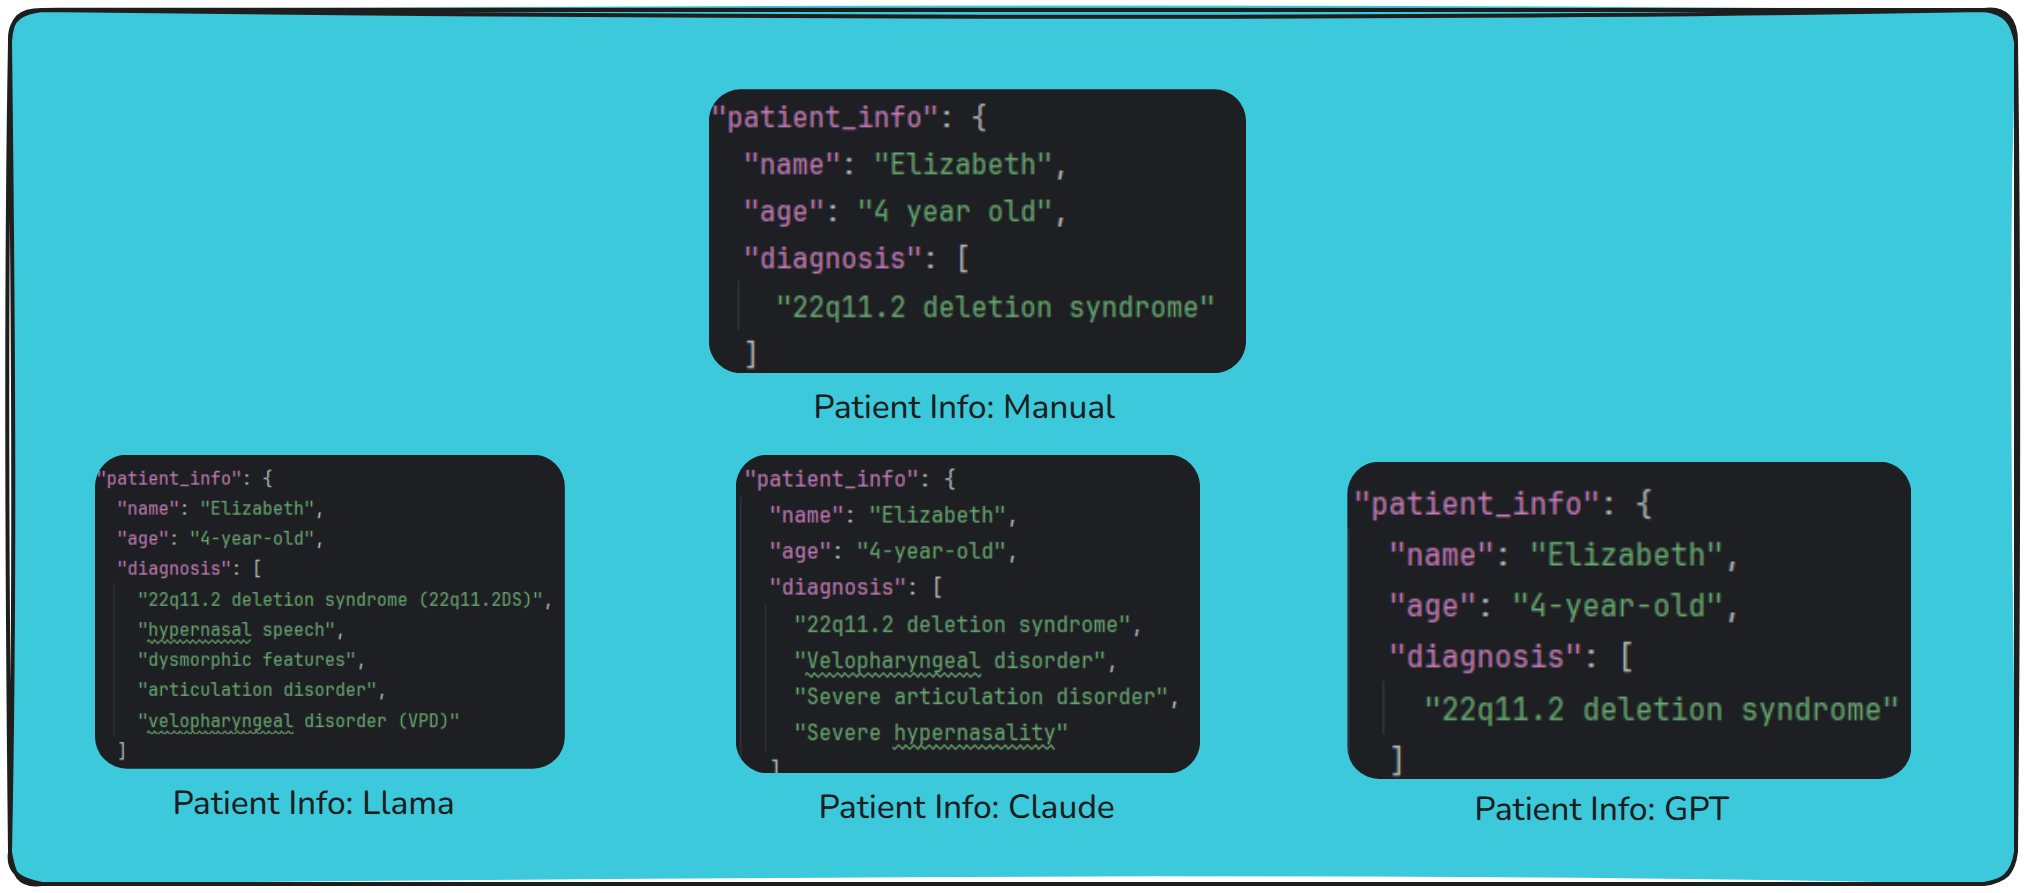
\includegraphics[width=1.0\textwidth]{Fig/Dataprep_patient_info.png}
    \caption{\centering Comparison of \texttt{patient\_info} field across manual, GPT-4o, Claude 3.5, and LLaMA 3.2}
    \label{fig:patient_info_comparison}
\end{figure}

The \texttt{patient\_info} field contains basic demographic and diagnostic details such as the patient’s name, age, and diagnosis. All three models successfully identified and extracted the patient's name as ``Elizabeth'' and represented the age as ``4-year-old,'' although Claude formatted it as ``4 year old'' (without hyphenation), and GPT preserved the format closest to the manual version.

The most noticeable difference appeared in the \texttt{diagnosis} field. The manually curated JSON included only one diagnosis: \texttt{"22q11.2 deletion syndrome"}. GPT-4o reproduced this faithfully, whereas Claude and LLaMA included additional inferred conditions such as ``severe hypernasality,'' ``velopharyngeal disorder,'' and ``articulation disorder.'' While these additions are medically plausible and contextually relevant, they are not explicitly mentioned in the original text, making them mild hallucinations.

Overall, GPT-4o most closely matched the manual version in both structure and content. Claude and LLaMA tended to be more verbose or inferential in their outputs, which may reflect an attempt to enrich the response but could introduce unintended interpretations if used in a strictly extractive setting.

\begin{figure}[H]
    \centering
    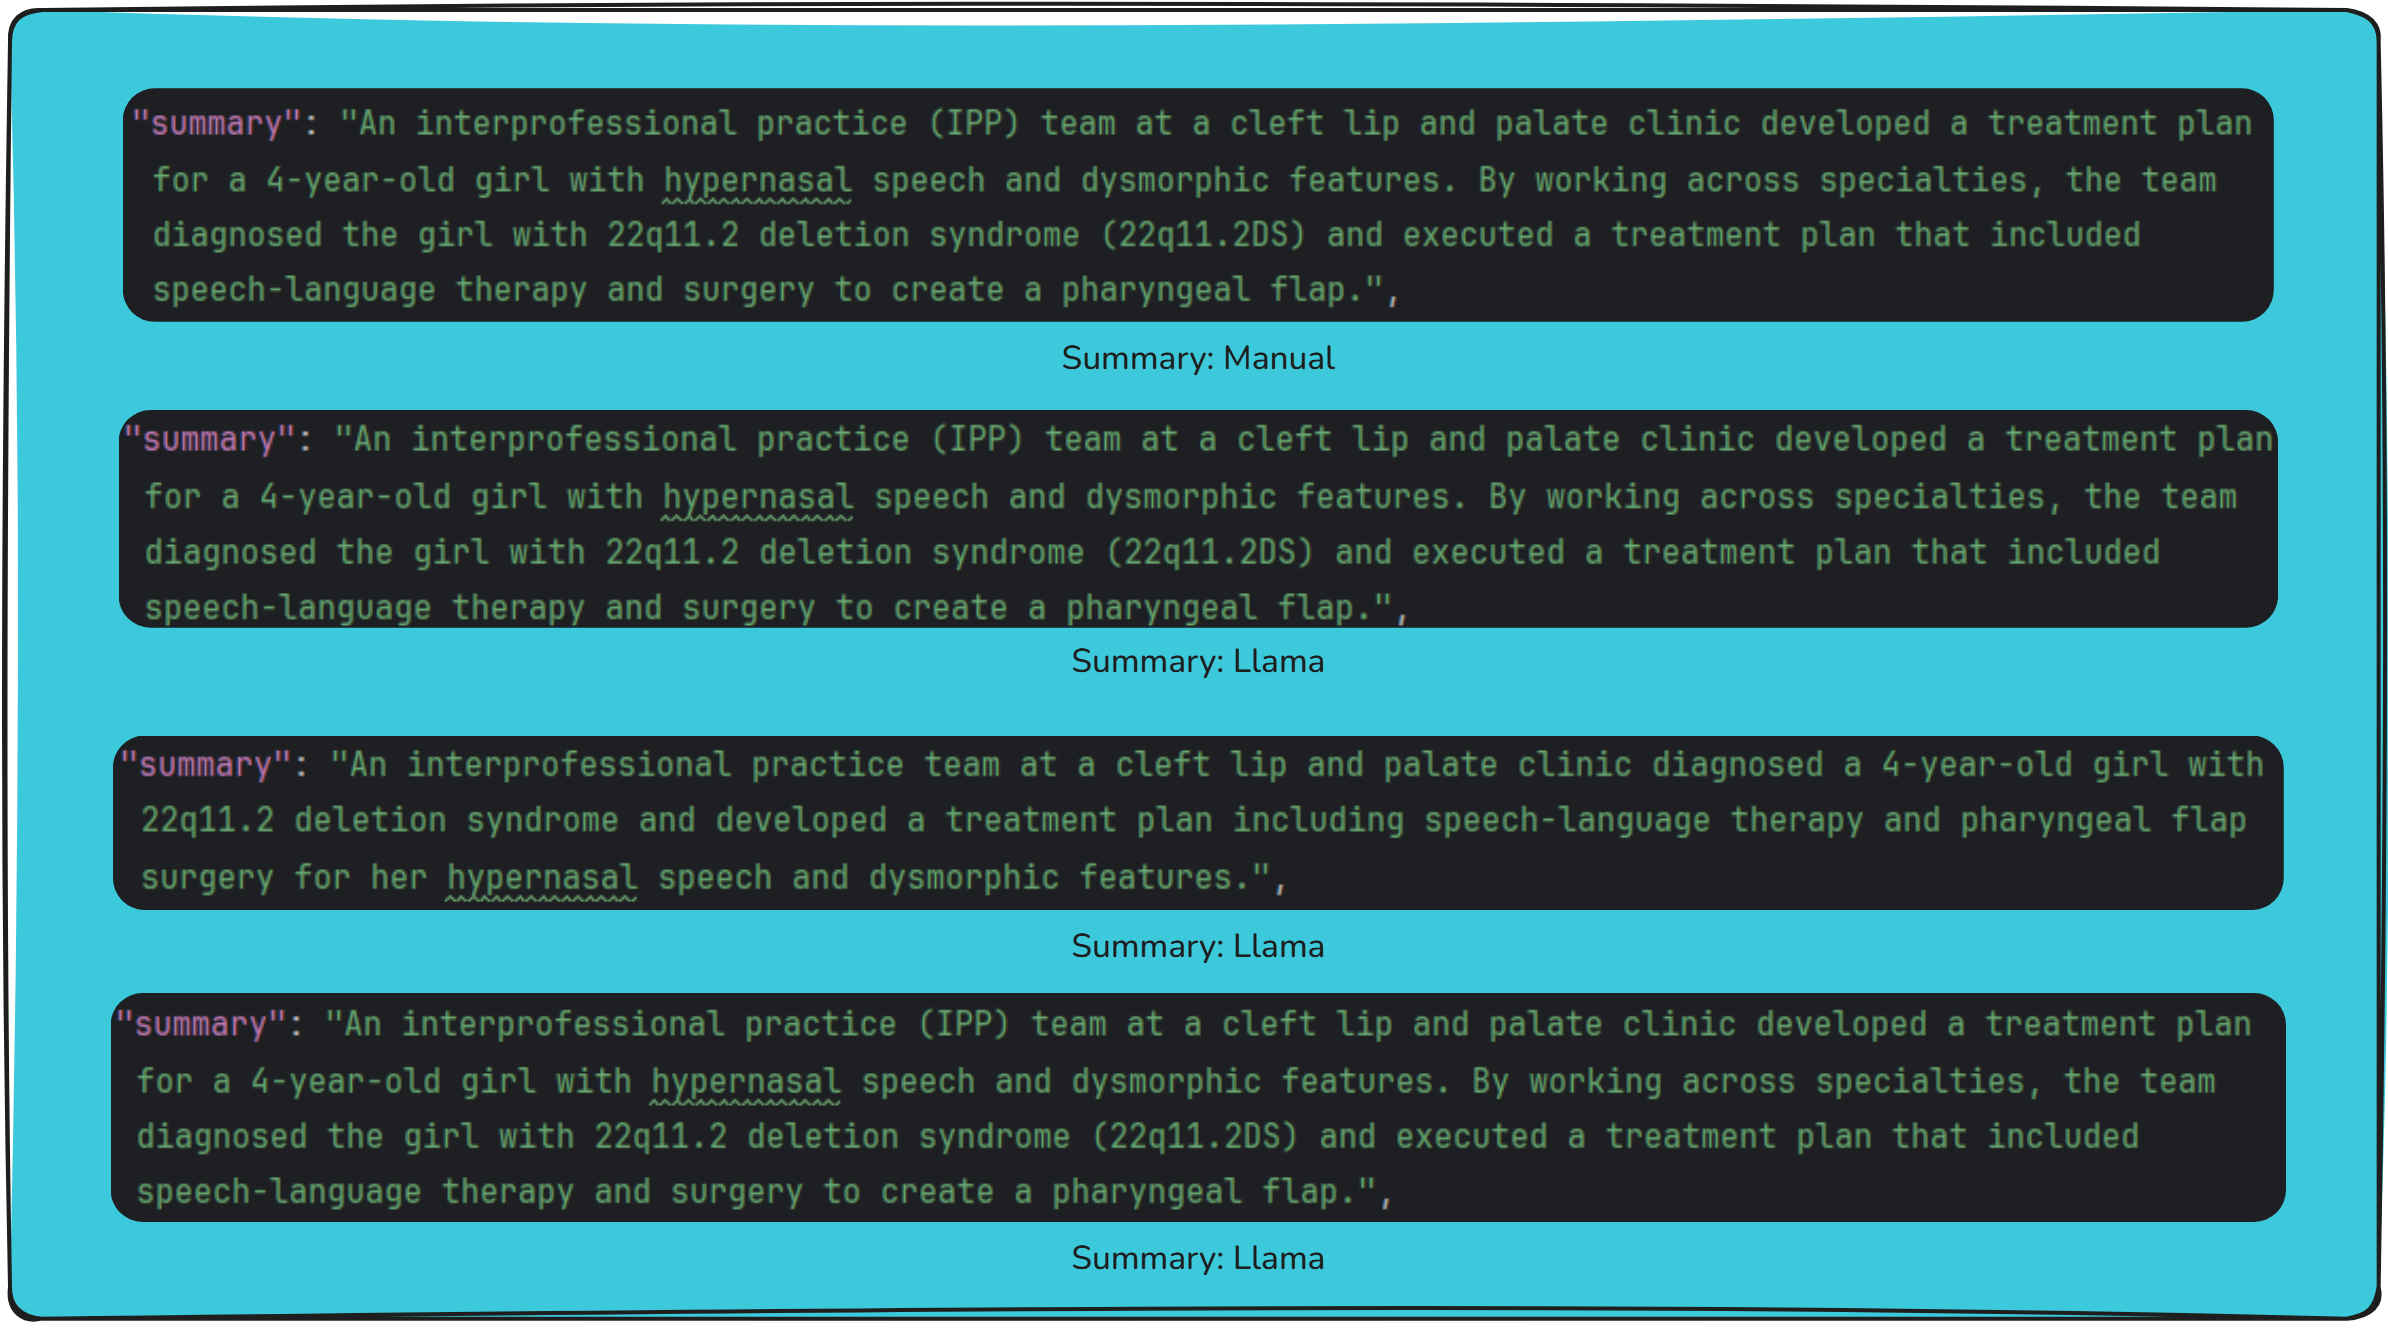
\includegraphics[width=1.0\textwidth]{Fig/Dataprep_summary.png}
    \caption{\centering Comparison of \texttt{summary} field across manual, GPT-4o, Claude 3.5, and LLaMA 3.2}
    \label{fig:summary_comparison}
\end{figure}

The \texttt{summary} field is intended to provide a concise, high-level overview of the case study. Both the manually extracted summary and the outputs from GPT-4o and LLaMA aligned closely in structure and wording, reflecting near-verbatim extraction of the original narrative.

Claude 3.5, however, restructured the sentence slightly, opting for a more natural and narrative-driven style. It preserved the core content but combined diagnosis and planned evaluation into a smoother, paraphrased form. While the meaning remained intact, the output lacked the more factual tone and field-oriented structure seen in the manual version.

This contrast highlights a key difference in model behavior: while GPT-4o and LLaMA tend to extract text conservatively, Claude occasionally leans toward stylistic fluency, which could be beneficial for summarization tasks but may diverge from strict extraction goals.

\begin{figure}[H]
    \centering
    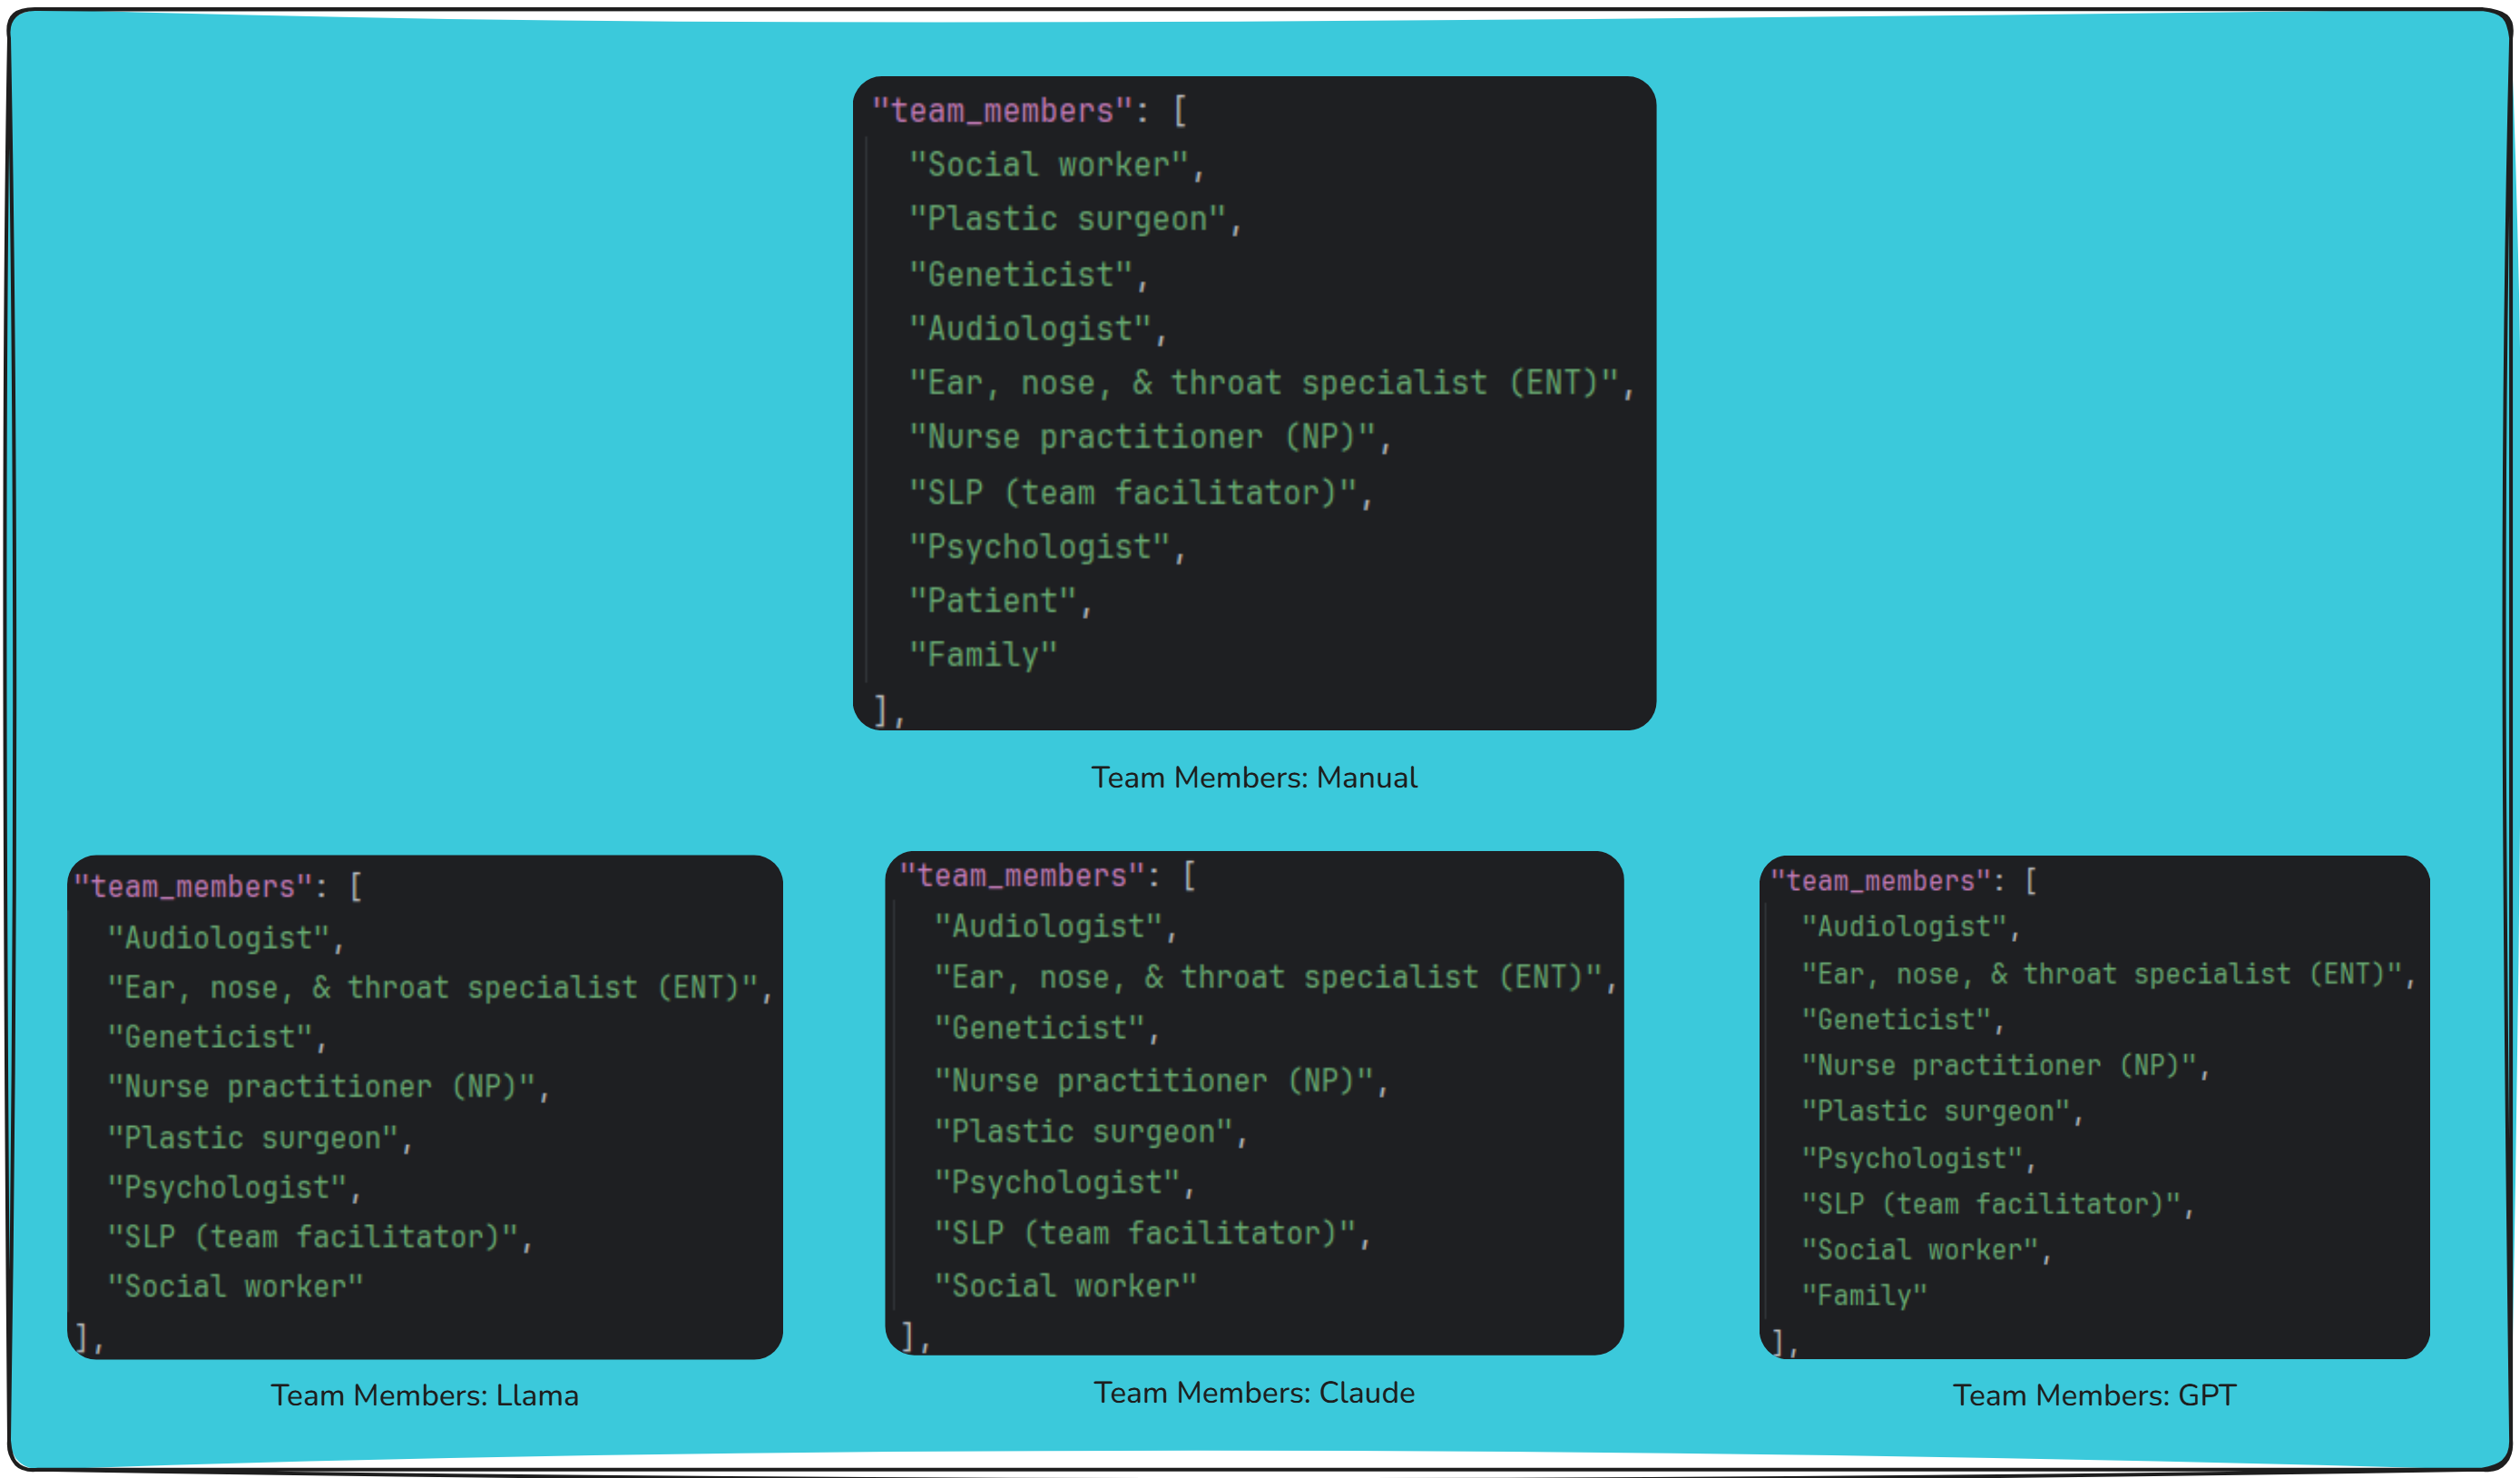
\includegraphics[width=1.0\textwidth]{Fig/Dataprep_team_members.png}
    \caption{\centering Comparison of \texttt{team\_members} field across manual, GPT-4o, Claude 3.5, and LLaMA 3.2}
    \label{fig:team_members_comparison}
\end{figure}

The \texttt{team\_members} field lists the various professionals and individuals involved in the patient’s care team. The manually curated JSON included all ten members explicitly mentioned in the case study, including both clinical professionals (e.g., speech-language pathologist, geneticist) and non-clinical roles (e.g., patient, family).

GPT-4o was the most faithful to the manual version, preserving the full list of team members without omissions. In contrast, both Claude and LLaMA excluded the ``Patient'' and ``Family'' roles from their outputs. This suggests that these models may be biased toward recognizing only formal clinical roles and may filter out perceived “non-professional” entries when summarizing or extracting data.

While this filtering may not affect downstream treatment generation in most cases, it does reflect a subtle divergence in how different models interpret the definition of a “team” in an interprofessional context—particularly important in domains like IPE, where holistic and family-centered care is emphasized.

\begin{figure}[H]
    \centering
    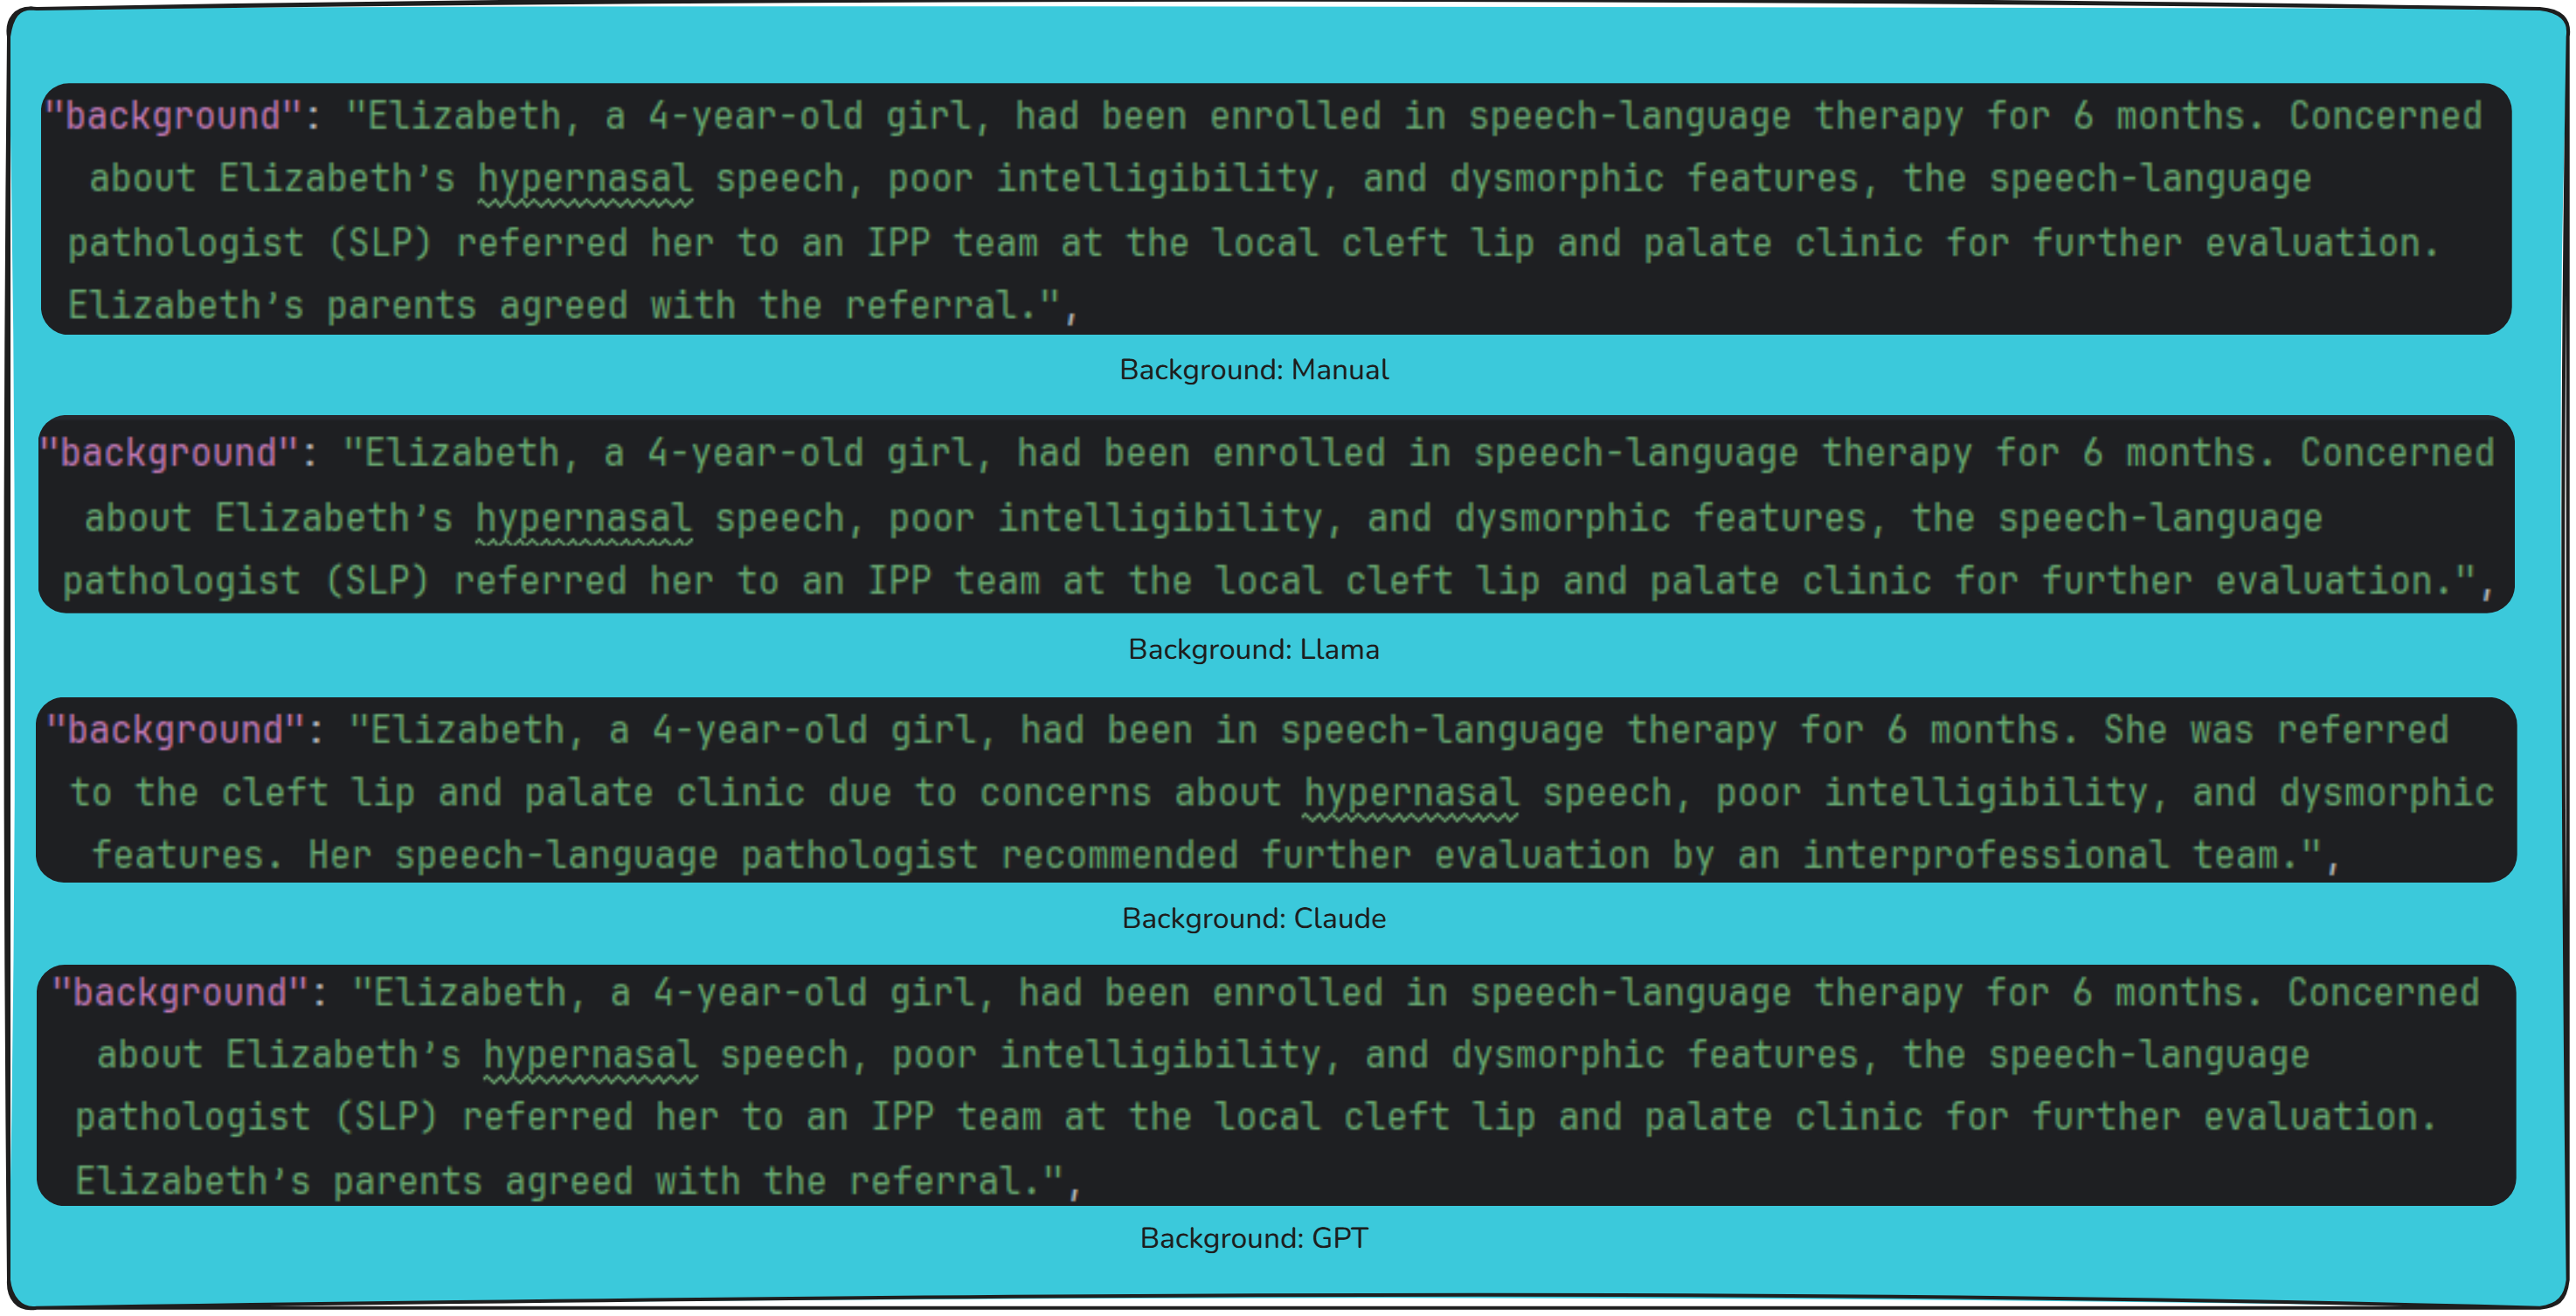
\includegraphics[width=1.0\textwidth]{Fig/Dataprep_background.png}
    \caption{\centering Comparison of \texttt{background} field across manual, GPT-4o, Claude 3.5, and LLaMA 3.2}
    \label{fig:background_comparison}
\end{figure}

The \texttt{background} field captures the patient’s clinical history and contextual information leading up to the current referral. All three LLMs extracted the key details from the source PDF with a high degree of fidelity, closely matching the manually curated version.

GPT-4o and LLaMA followed the source phrasing quite literally, maintaining the sentence structure and terminology with minimal deviation. Claude 3.5 introduced a small stylistic change by paraphrasing part of the referral statement—transforming ``The patient was referred...'' into ``Evaluation was recommended...''—which slightly alters the tone but not the factual content.

This field showed the most consistency across models, suggesting that straightforward narrative segments with minimal ambiguity are well-handled by all three LLMs when structured prompting is applied.

\begin{figure}[H]
    \centering
    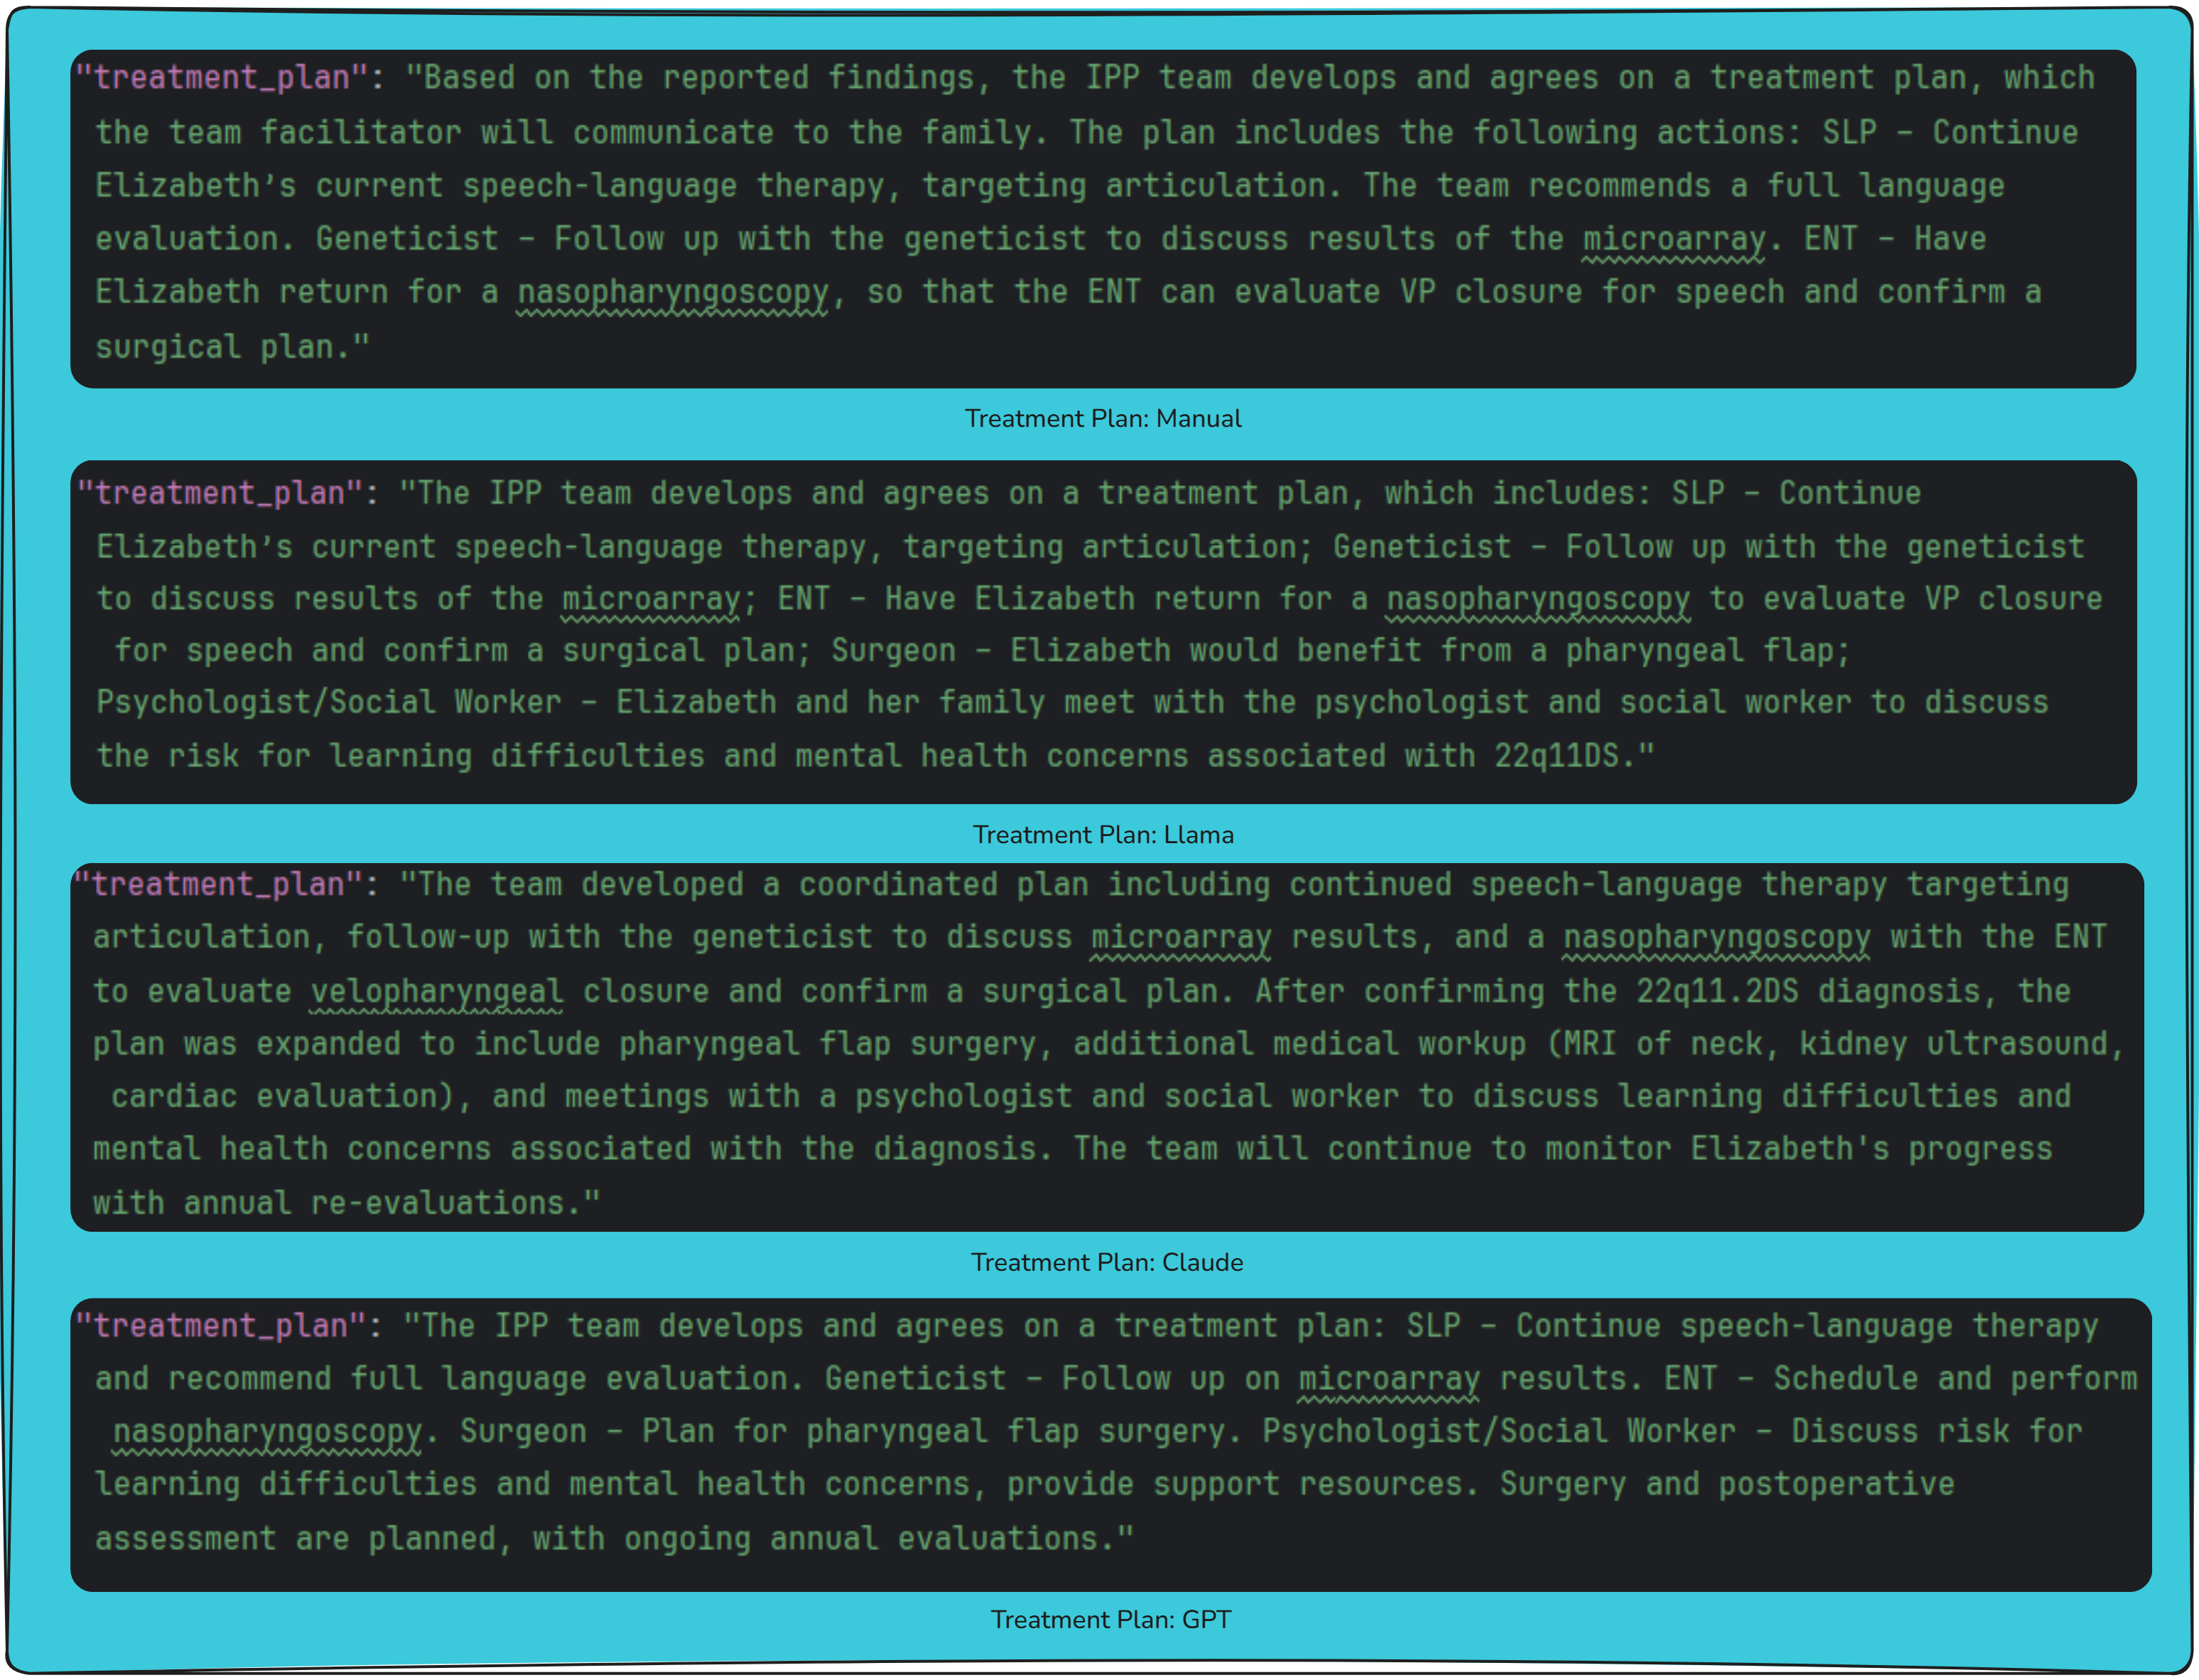
\includegraphics[width=1.0\textwidth]{Fig/Dataprep_treatment_plan.png}
    \caption{\centering Comparison of \texttt{treatment\_plan} field across manual, GPT-4o, Claude 3.5, and LLaMA 3.2}
    \label{fig:treatment_plan_comparison}
\end{figure}

The \texttt{treatment\_plan} field represents the most complex and interpretive portion of the extracted data, as it aggregates recommendations from multiple interprofessional team members. The manually prepared version offers a clean breakdown with clearly delineated contributions from each role.

GPT-4o generated a concise and reasonably structured plan, correctly identifying most team members and assigning plausible actions. However, its output was relatively short and omitted several role-specific recommendations found in the manual version.

LLaMA and Claude 3.5 produced significantly longer and more detailed outputs. Both captured additional tasks, such as ``long-term hearing monitoring'' or ``referrals for social support,'' which were not explicitly stated in the case study but are contextually relevant. While this can add richness, it also introduces interpretive variability and potential hallucinations.

Notably, both LLaMA and Claude reformatted the original structure into more prose-driven responses rather than following the explicit team-member formatting in the manual. This divergence highlights the models’ tendency to favor generative fluency over strict structural alignment when not explicitly instructed to follow a rigid schema.
Overall, all three models successfully conveyed the core components of the treatment plan, but their outputs varied significantly in verbosity, structure, and interpretive scope.

Across the five fields examined—\texttt{patient\_info}, \texttt{summary}, \texttt{team\_members}, \texttt{background}, and \texttt{treatment\_plan}—all three LLMs demonstrated the ability to extract structured information from unstructured clinical narratives with varying levels of fidelity. GPT-4o tended to preserve original phrasing and structure more faithfully, while Claude 3.5 and LLaMA 3.2 occasionally introduced additional content or reformatted outputs in more narrative styles. Although some outputs included minor hallucinations or omitted less obvious roles, the core medical context was retained in all cases.

Ultimately, the qualitative differences observed across models were not significant enough to impact downstream performance in treatment plan generation. This supports our decision to use the LLM-specific extracted JSONs as valid input for subsequent evaluation stages, without the need for strict quantitative scoring or error correction.




\subsection{Treatment Plans comparision - OpenAI vs Claude vs Llama}\label{subsec4.3}
\subsubsection{Manually prepared data}\label{subsec4.3.1}
\subsubsection{LLM prepared data}\label{subsec4.3.2}
\subsection{ LLM vs Prompt Tuned LLM vs MediSyn}\label{subsec4.4}
\subsubsection{Manually prepared data}\label{subsec4.4.1}
\subsubsection{LLM prepared data}\label{subsec4.4.2}


\section{Discussion and Limitations}\label{sec5}

\section{Conclusion}\label{sec6}

\section*{Data Availability}
The authors confirm that the datasets generated during and/or analyzed during the current study are available from the corresponding author on reasonable request.



\bmhead{Supplementary information}

If your article has accompanying supplementary file/s please state so here. 

Authors reporting data from electrophoretic gels and blots should supply the full unprocessed scans for key as part of their Supplementary information. This may be requested by the editorial team/s if it is missing.

Please refer to Journal-level guidance for any specific requirements.

\bmhead{Acknowledgements}

Acknowledgements are not compulsory. Where included they should be brief. Grant or contribution numbers may be acknowledged.

Please refer to Journal-level guidance for any specific requirements.

\section*{Declarations}

Some journals require declarations to be submitted in a standardised format. Please check the Instructions for Authors of the journal to which you are submitting to see if you need to complete this section. If yes, your manuscript must contain the following sections under the heading `Declarations':

\begin{itemize}
\item Funding
\item Conflict of interest/Competing interests (check journal-specific guidelines for which heading to use)
\item Ethics approval and consent to participate
\item Consent for publication
\item Data availability 
\item Materials availability
\item Code availability 
\item Author contribution
\end{itemize}

\noindent
If any of the sections are not relevant to your manuscript, please include the heading and write `Not applicable' for that section. 

%%===================================================%%
%% For presentation purpose, we have included        %%
%% \bigskip command. Please ignore this.             %%
%%===================================================%%
\bigskip
\begin{flushleft}%
Editorial Policies for:

\bigskip\noindent
Springer journals and proceedings: \url{https://www.springer.com/gp/editorial-policies}

\bigskip\noindent
Nature Portfolio journals: \url{https://www.nature.com/nature-research/editorial-policies}

\bigskip\noindent
\textit{Scientific Reports}: \url{https://www.nature.com/srep/journal-policies/editorial-policies}

\bigskip\noindent
BMC journals: \url{https://www.biomedcentral.com/getpublished/editorial-policies}
\end{flushleft}

\begin{appendices}

\section{Section title of first appendix}\label{secA1}

An appendix contains supplementary information that is not an essential part of the text itself but which may be helpful in providing a more comprehensive understanding of the research problem or it is information that is too cumbersome to be included in the body of the paper.

%%=============================================%%
%% For submissions to Nature Portfolio Journals %%
%% please use the heading ``Extended Data''.   %%
%%=============================================%%

%%=============================================================%%
%% Sample for another appendix section			       %%
%%=============================================================%%

%% \section{Example of another appendix section}\label{secA2}%
%% Appendices may be used for helpful, supporting or essential material that would otherwise 
%% clutter, break up or be distracting to the text. Appendices can consist of sections, figures, 
%% tables and equations etc.

\end{appendices}

%%===========================================================================================%%
%% If you are submitting to one of the Nature Portfolio journals, using the eJP submission   %%
%% system, please include the references within the manuscript file itself. You may do this  %%
%% by copying the reference list from your .bbl file, paste it into the main manuscript .tex %%
%% file, and delete the associated \verb+\bibliography+ commands.                            %%
%%===========================================================================================%%

\bibliography{sn-bibliography}% common bib file
%% if required, the content of .bbl file can be included here once bbl is generated
%%\input sn-article.bbl

\end{document}
